\documentclass[main.tex]{subfiles}
\begin{document}

\href{https://www2.seas.gwu.edu/~simhaweb/quantum/modules/module5/module5.html}{Module 5: Multiple Qubits - Measurement and Modification}

\subsection{A brief review of projections}

    Let's first examine projections with real vectors: Suppose $V$ is a space with basis $\left|e_{1}\right\rangle, \ldots,\left|e_{n}\right\rangle$. Within $V$ suppose $\left|v_{1}\right\rangle,\left|v_{2}\right\rangle$ are orthonormal vectors. Then,
    
    $$
    V_{1}=\operatorname{span}\left\{\left|v_{1}\right\rangle,\left|v_{2}\right\rangle\right\}
    $$
    
    is a subspace of $V$ : Any $\alpha_{1}\left|v_{1}\right\rangle+\alpha_{2}\left|v_{2}\right\rangle$ is in $V_{1}$. But there are vectors in $V$ not in $V_{1}$. Let $|w\rangle$ be any vector in $V$ (the larger space). Then consider the projection of $|w\rangle$ on span $\left\{\left|v_{1}\right\rangle,\left|v_{2}\right\rangle\right\}$ shown in Figure \ref{fig:01projection}.
    
    \begin{figure}
        \centering
        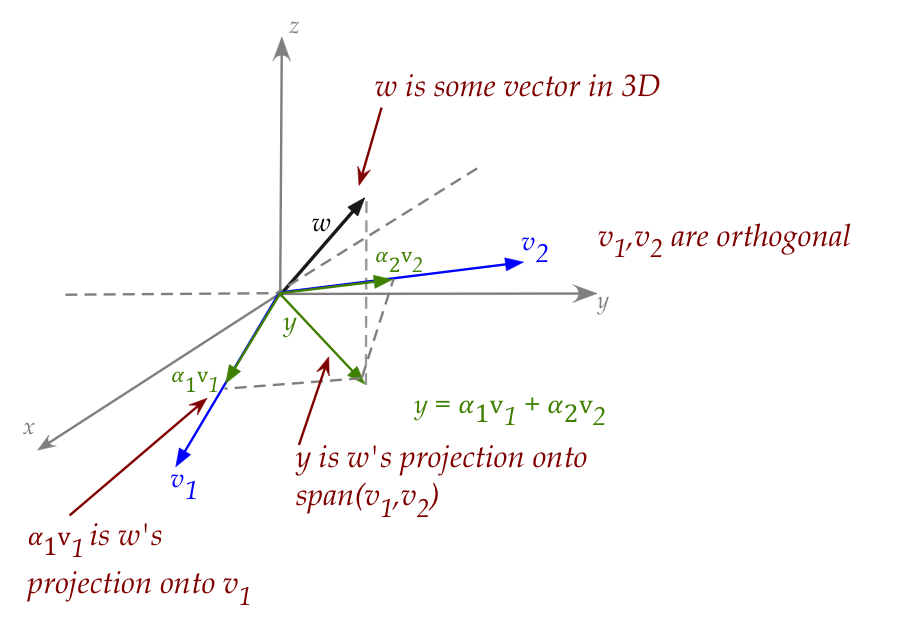
\includegraphics[width=4in]{notes/figs/n07/01projection.png}
        \caption{Projection}
        \label{fig:01projection}
    \end{figure} 
    
    Observe the following in the figure: Here, span $\left\{\left|v_{1}\right\rangle,\left|v_{2}\right\rangle\right\}$ is the $\mathrm{x}-\mathrm{y}$ plane. The projection of $|w\rangle$ is the shadow it casts on the $x$-y plane, which we've called $|y\rangle$. $|w\rangle$ has projections on the individual vectors $\left|v_{1}\right\rangle$ and $\left|v_{2}\right\rangle$ :
    
    $$
    \begin{aligned}
    &\alpha_{1}\left|v_{1}\right\rangle=\text { Projection of }|w\rangle \text { along }\left|v_{1}\right\rangle \\
    &\alpha_{2}\left|v_{2}\right\rangle=\text { Projection of }|w\rangle \text { along }\left|v_{1}\right\rangle
    \end{aligned}
    $$
    
    Because $\left|v_{1}\right\rangle,\left|v_{2}\right\rangle$ are orthogonal, the sum of these projections is $|y\rangle$ :
    
    $$
    |y\rangle=\alpha_{1}\left|v_{1}\right\rangle+\alpha_{2}\left|v_{2}\right\rangle
    $$
    
    (The parallelogram is a rectangle). We'll now thoroughly exploit the simplifications that arise from unit-length and orthogonality. First, recall: the coefficients $\alpha_{1}, \alpha_{2}$ are merely inner-products:
    
    $$
    \alpha_{i}=\left\langle v_{i} \mid w\right\rangle
    $$
    
    And the projected vectors can be obtained by applying projectors:
    
    $$
    \alpha_{i}\left|v_{i}\right\rangle=\left|v_{i}\right\rangle\left\langle v_{i}|| w\right\rangle=\left(\left\langle v_{i} \mid w\right\rangle\right)\left|v_{i}\right\rangle
    $$
    
    Thus, we can build a combined single projector for the subspace $V_{1}$ by adding the two projectors:
    
    $$
    \begin{aligned}
    \left(\left|v_{1}\right\rangle\left\langle v_{1}|+| v_{2}\right\rangle\left\langle v_{2}\right|\right)|w\rangle &=\left|v_{1}\right\rangle\left\langle v_{1}|| w\right\rangle+\left|v_{2}\right\rangle\left\langle v_{2}|| w\right\rangle \\
    &=\left|v_{1}\right\rangle\left\langle v_{1} \mid w\right\rangle+\left|v_{2}\right\rangle\left\langle v_{2} \mid w\right\rangle \\
    &=\left(\left\langle v_{1} \mid w\right\rangle\right)\left|v_{1}\right\rangle+\left(\left\langle v_{2} \mid w\right\rangle\right)\left|v_{2}\right\rangle \\
    &=\left(\alpha_{1}\right)\left|v_{1}\right\rangle+\left(\alpha_{2}\right)\left|v_{2}\right\rangle \\
    &=|y\rangle
    \end{aligned}
    $$
    
    Although we used real vectors, everything we've described applies to complex vectors.

\subsection{Projective measurement: what's needed for multiple qubits}

    Let's start by reviewing, via an example, how projective measurement worked for the single qubit: Recall, there are four steps: 1 . Identify the projectors for the basis:
    
    $$
    P_{i}=\left|v_{i}\right\rangle\left\langle v_{i}\right|
    $$
    
    2. Compute each projected vector:
    
    $$
    \left|\psi_{P_{i}}\right\rangle=P_{i}|\psi\rangle
    $$
    
    3. Compute the squared magnitude of each projection: ||$\left.\psi_{P_{i}}\right\rangle\left.\right|^{2}$ as the probability of seeing the i-th normalized projection. 4. Compute each normalized projection (each potential outcome):
    
    $$
    \left|\psi_{N_{i}}\right\rangle=\frac{\left|\psi_{P_{i}}\right\rangle}{\left.\| \psi_{P_{i}}\right\rangle \mid}
    $$
    
    This gives us each possible outcome and its associated probability: Outcome $\left|\psi_{N_{i}}\right\rangle$ occurs with probability ||$\left.\psi_{P_{i}}\right\rangle\left.\right|^{2}$. For example, suppose we measure $|0\rangle$ in the basis $|+\rangle,|-\rangle$. Step 1: Identify the projectors for the basis.
    
    $$
    \begin{aligned}
    &\left.P_{+}=1+\right\rangle\langle+1 \\
    &\left.P_{-}=1-\right\rangle\langle-1
    \end{aligned}
    $$
    
    Step 2: Compute each projected vector:
    
    $$
    \begin{aligned}
    &\left.P_{+}|0\rangle=|+\rangle\langle+|| 0\rangle=1+\right\rangle\left\langle+\left|\left(\frac{1}{\sqrt{2}}|+\rangle+\frac{1}{\sqrt{2}}|-\rangle\right)=\frac{1}{\sqrt{2}}\right|+\right\rangle \\
    &P_{-}|0\rangle=|-\rangle\langle-|| 0\rangle=|-\rangle\left\langle-\left|\left(\frac{1}{\sqrt{2}}|+\rangle+\frac{1}{\sqrt{2}}|-\rangle\right)=\frac{1}{\sqrt{2}}\right|-\right\rangle
    \end{aligned}
    $$
    
    (Recall: $\left.|0\rangle=\frac{1}{\sqrt{2}}|+\rangle+\frac{1}{\sqrt{2}}|-\rangle\right)$ Step 3: Compute the squared magnitude of each projection:
    
    $$
    \begin{aligned}
    &\left.\left.\left|P_{+}\right| 0\right\rangle\left.\right|^{2}=\left|\frac{1}{\sqrt{2}}\right|+\right\rangle\left.\right|^{2}=\left\langle\frac{1}{\sqrt{2}}\left\langle+|| \frac{1}{\sqrt{2}} \mid+\right\rangle\right\rangle=\frac{1}{2} \\
    &\left.\left.\left|P_{-}\right| 0\right\rangle\left.\right|^{2}=\left|\frac{1}{\sqrt{2}}\right|-\right\rangle\left.\right|^{2}=\left\langle\frac{1}{\sqrt{2}}\left\langle-|| \frac{1}{\sqrt{2}} \mid-\right\rangle\right\rangle=\frac{1}{2}
    \end{aligned}
    $$
    
    Step 4: Compute each normalized projection (each potential outcome):
    
    $$
    \begin{aligned}
    &\frac{\frac{1}{\sqrt{2}}|+\rangle}{\left.\left|\frac{1}{\sqrt{2}}\right|+\right\rangle \mid}=|+\rangle \\
    &\frac{\frac{1}{\sqrt{2}}|-\rangle}{\left.\left|\frac{1}{\sqrt{2}}\right|-\right\rangle \mid}=|-\rangle
    \end{aligned}
    $$
    
    This gives us possible outcomes and their associated probabilities:
    
    $$
    \begin{array}{ll}
    \text { outcome }|+\rangle \text { occurs with probability } & \frac{1}{2} \\
    \text { outcome }|-\rangle \text { occurs with probability } & \frac{1}{2}
    \end{array}
    $$
    
    Now, we could have inferred these directly by examining the target vector expressed in the measurement basis: Express $|0\rangle$ in the $|+\rangle,|-\rangle$ basis:
    
    $$
    |0\rangle=\frac{1}{\sqrt{2}}|+\rangle+\frac{1}{\sqrt{2}}|-\rangle
    $$
    
    Then, the probability of observing $|+\rangle$, is just
    
    $$
    \left|\frac{1}{\sqrt{2}}\right|^{2}=\frac{1}{2}
    $$
    
    Thus, the extra trouble of projective measurement is often overkill for a single qubit. Now let's examine projective measurement with two qubits: It's here that we run into a complication as shown in Figure \ref{fig:02measure1}.

    \begin{figure}
        \centering
        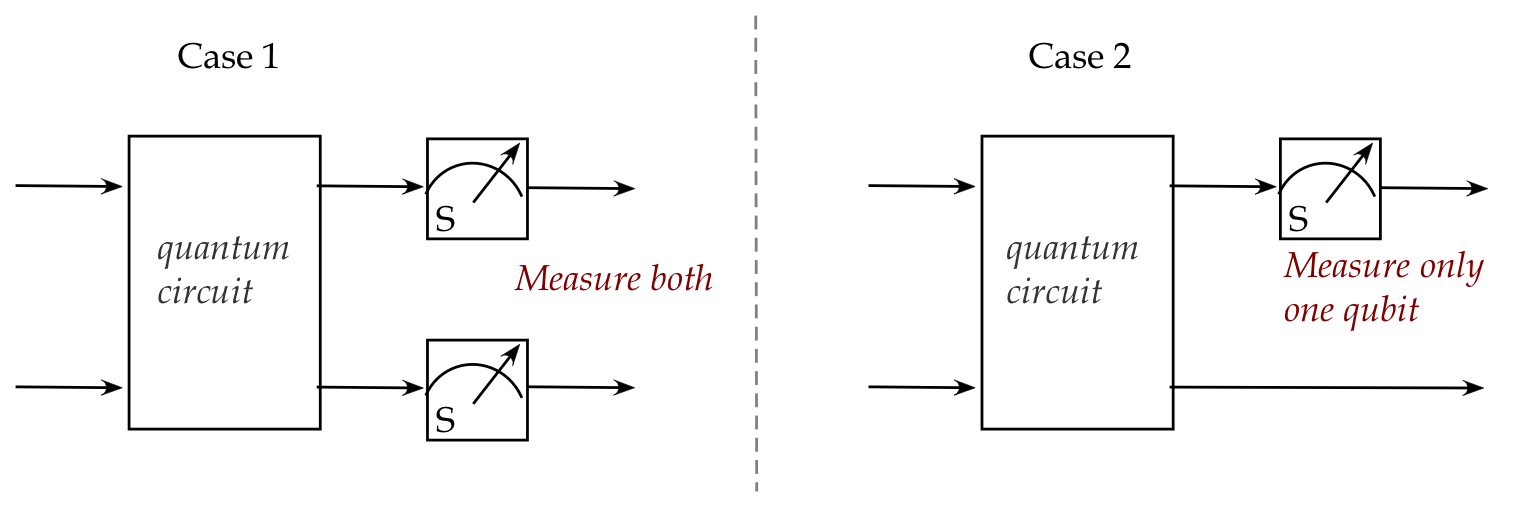
\includegraphics[width=4in]{notes/figs/n07/02measure1.png}
        \caption{Possible to measure one qubit?}
        \label{fig:02measure1}
    \end{figure} 
    
    Are both qubits to be measured together? Is it possible to measure just one qubit? A second complication: how do we reason about the case when two qubits are apart as shown in Figure \ref{fig:03measure2}.
    
    \begin{figure}
        \centering
        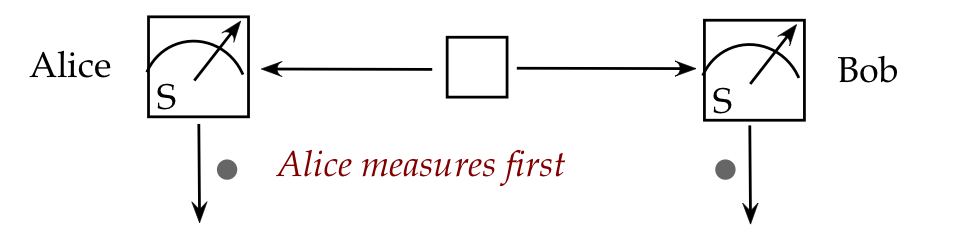
\includegraphics[width=4in]{notes/figs/n07/03measure2.png}
        \caption{When two qubits are apart}
        \label{fig:03measure2}
    \end{figure} 
    
    Let's examine two-qubits-together with an example: Consider the two-qubit state
    
    $$
    |\psi\rangle=\frac{1}{\sqrt{2}}|01\rangle+\frac{1}{\sqrt{2}}|10\rangle
    $$
    
    And suppose we use the two-qubit standard basis for two-qubit measurement:
    
    $$
    |00\rangle, \quad|01\rangle_{+} \quad|10\rangle, \quad|11\rangle
    $$
    
    First consider the direct approach: The outcomes of measurement are the measurement-basis vectors: $|00\rangle,|01\rangle,|10\rangle,|11\rangle$. We now express the vector $|\psi\rangle$ in the measurement basis:
    
    $$
    |\psi\rangle=0|00\rangle+\frac{1}{\sqrt{2}}|01\rangle+\frac{1}{\sqrt{2}}|10\rangle+0|11\rangle
    $$
    
    Thus: $|00\rangle$ occurs with probability 0, $|01\rangle$ occurs with probability $\left|\frac{1}{\sqrt{2}}\right|^{2}$, $|10\rangle$ occurs with probability $\left|\frac{1}{\sqrt{2}}\right|^{2}$ |11) occurs with probability 0. Next, let's see how this works with projective measurement: Step 1: Identify the measurement basis projectors:
    
    $$
    \begin{aligned}
    &P_{00}=|00\rangle\langle 00| \\
    &P_{01}=|01\rangle\langle 01| \\
    &P_{10}=|10\rangle\langle 10| \\
    &P_{11}=|11\rangle\langle 11|
    \end{aligned}
    $$
    
    Step 2: Use the above to compute projected vectors:
    
    $$
    \begin{aligned}
    P_{00}|\psi\rangle &=|00\rangle\left\langle0 0 \left|\left(\frac{1}{\sqrt{2}}|01\rangle+\frac{1}{\sqrt{2}}|10\rangle\right)=0\right.\right.\\
    P_{01}|\psi\rangle &=|01\rangle\left\langle 01\left|\left(\frac{1}{\sqrt{2}}|01\rangle+\frac{1}{\sqrt{2}}|10\rangle\right)=\frac{1}{\sqrt{2}}\right| 01\right\rangle \\
    P_{10}|\psi\rangle &=|10\rangle\left\langle 10\left|\left(\frac{1}{\sqrt{2}}|01\rangle+\frac{1}{\sqrt{2}}|10\rangle\right)=\frac{1}{\sqrt{2}}\right| 10\right\rangle \\
    P_{11}|\psi\rangle &=|11\rangle\left\langle1 1 \left|\left(\frac{1}{\sqrt{2}}|01\rangle+\frac{1}{\sqrt{2}}|10\rangle\right)=0\right.\right.
    \end{aligned}
    $$
    
    Step 3: The magnitudes of (non-zero) projected vectors are their probabilities:
    
    $$
    \begin{aligned}
    \left.\left|P_{01}\right| \psi\right\rangle\left.\right|^{2} &\left.=\left|\frac{1}{\sqrt{2}}\right| 01\right\rangle\left.\right|^{2}=\frac{1}{2} \\
    \left.\left|P_{10}\right| \psi\right\rangle\left.\right|^{2} &\left.=\left|\frac{1}{\sqrt{2}}\right| 10\right\rangle\left.\right|^{2}=\frac{1}{2}
    \end{aligned}
    $$
    
    Step 4: Normalize the projections to get the outcome vectors:
    
    $$
    \begin{aligned}
    &\frac{1}{\left.\left|P_{01}\right| \psi\right\rangle \mid} P_{01}|\psi\rangle=|01\rangle \\
    &\frac{1}{\left.\left|P_{10}\right| \psi\right\rangle \mid} P_{10}|\psi\rangle=|10\rangle
    \end{aligned}
    $$
    
    Notice the usefulness of Dirac notation in the second step, for example reference Figure \ref{fig:04measure3}.
    
    \begin{figure}
        \centering
        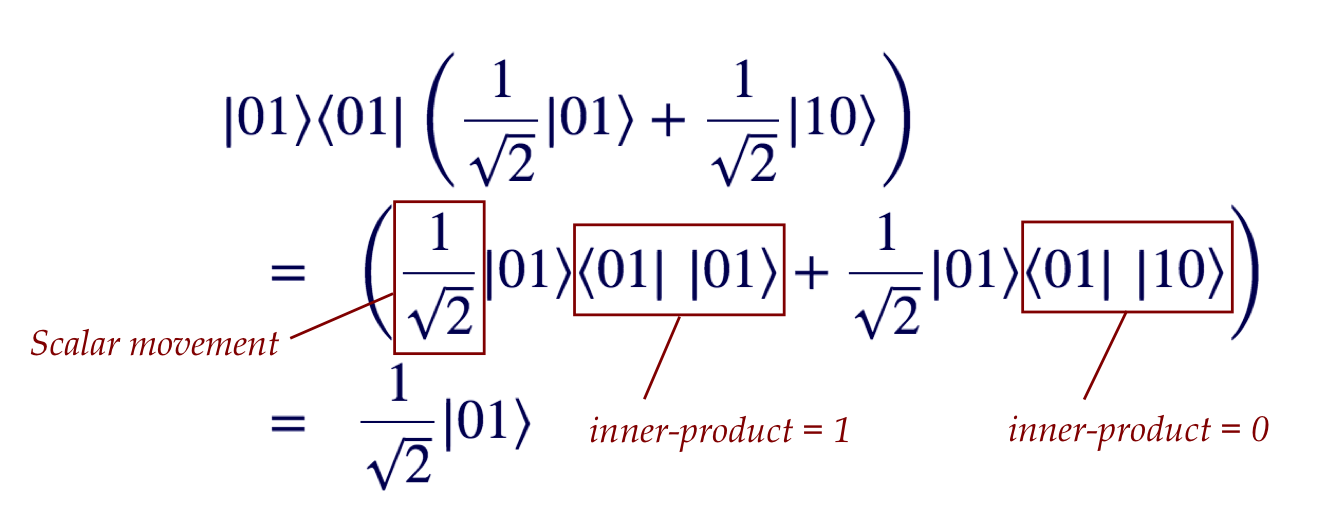
\includegraphics[width=4in]{notes/figs/n07/04measure3.png}
        \caption{Dirac notation utility}
        \label{fig:04measure3}
    \end{figure} 
    
    At this point, projective measurement still seems like overkill. Now suppose we want to measure only the first qubit referenced in Figure \ref{fig:05measure4}.
    
    \begin{figure}
        \centering
        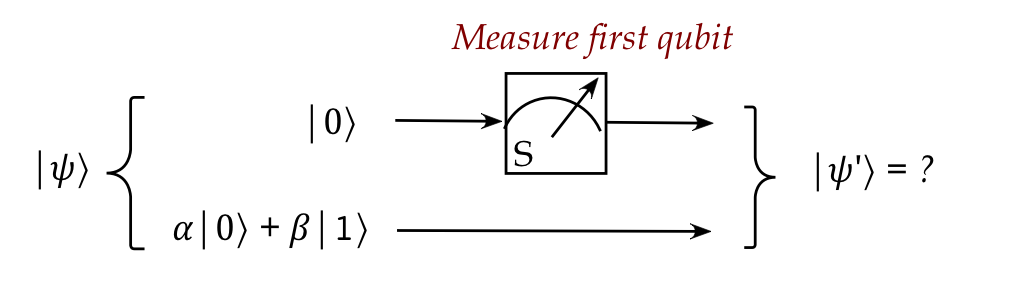
\includegraphics[width=4in]{notes/figs/n07/05measure4.png}
        \caption{Measure first qubit}
        \label{fig:05measure4}
    \end{figure} 
    
    Suppose the input two-qubit vector is
    
    $$
    |\psi\rangle=|0\rangle \otimes(\alpha|0\rangle+\beta|1\rangle)
    $$
    
    We'd like to know: after measuring only the first qubit, what are the possible states, and with what probabilities? Clearly, since the first (top) qubit is already $|0\rangle$, measuring this qubit alone should leave the top qubit as $|0\rangle$. Intuition suggests that because there's no entanglement, the second qubit should be the same. That is, after measurement, that state should be
    
    $$
    |\psi\rangle=|0\rangle \otimes(\alpha|0\rangle+\beta|1\rangle)
    $$
    
    In this case, we can apply tensoring rules to see that
    
    $$
    |\psi\rangle=\alpha(|0\rangle \otimes|0\rangle)+\beta(|0\rangle \otimes|1\rangle)=\alpha|00\rangle+\beta|01\rangle
    $$
    
    Any two-qubit measurement will leave the state either in $|00\rangle$ or $|01\rangle$. Thus, the two types of measurements produce different results, and we need to extend the theory to account for this. Next, consider what happens if the two-qubit state is entangled as shown in Figure \ref{fig:06measure5}.
    
    \begin{figure}
        \centering
        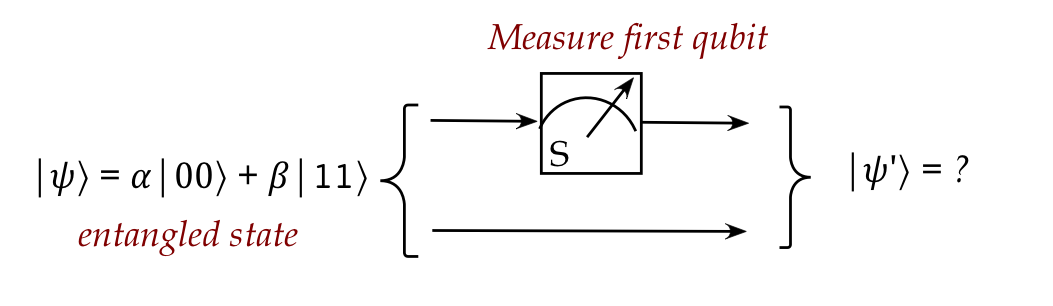
\includegraphics[width=4in]{notes/figs/n07/06measure5.png}
        \caption{Measure first qubit}
        \label{fig:06measure5}
    \end{figure}
    
    Here,
    
    $$
    |\psi\rangle=\alpha|00\rangle+\beta|11\rangle
    $$
    
    Intuitively, a first-qubit measurement should leave the state either in $|00\rangle$ or $|11\rangle$ with probabilities: 
    
    $$\begin{array}{ll}\text { outcome }|00\rangle & \text { with probability }|\alpha|^{2} \\ \text { outcome }|11\rangle & \text { with probability }|\beta|^{2}\end{array}$$. 
    
    How, then, should we reason about these different scenarios? Fortunately, projective measurement is easily extended to handle these cases.
    
\subsection{Projective measurement: extending the theory to multiple qubits}

    We want to extend the theory to be able to handle different measurement scenarios with $n$ qubits. Examples of scenarios include: Measuring all $n$ qubits simultaneously. Measuring just one qubit amongst the $n$ qubits. Measuring a subset of qubits from the $n$ qubits. And each case, having the freedom to use a variety of measurement bases. There are three aspects to extending single-qubit projective measurement to multiple qubits: Understanding how the particular measurement splits the whole $n$-qubit space into orthogonal subspaces. Building $n$-qubit projectors accordingly. Seeing if it helps to construct the $n$-qubit projectors from smaller projectors (such as 1-qubit projectors). Let's examine these aspects via a 2-qubit example shown in Figure \ref{fig:07measure6}.
    
    \begin{figure}
        \centering
        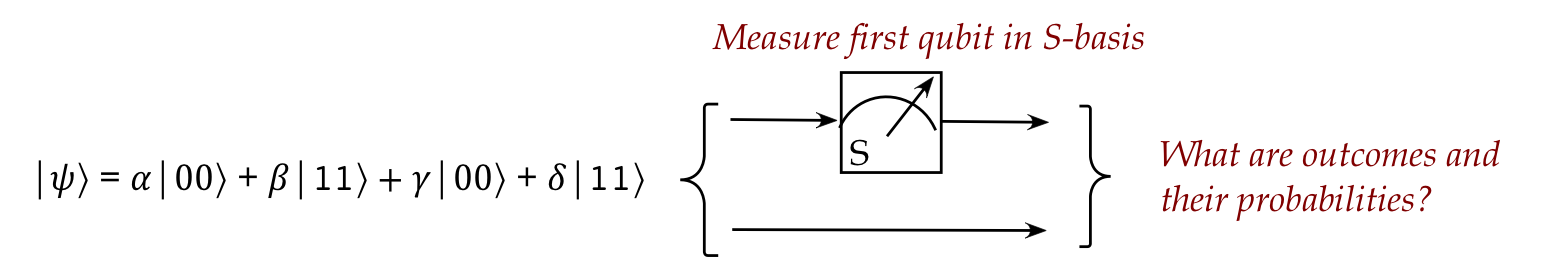
\includegraphics[width=4in]{notes/figs/n07/07measure6.png}
        \caption{Measure first qubit in S-basis}
        \label{fig:07measure6}
    \end{figure}
    
    Here, the input is a general 2-qubit vector
    
    $$
    |\psi\rangle=\alpha|00\rangle+\beta|01\rangle+\gamma|10\rangle+\delta|11\rangle
    $$
    
    We're measuring the top qubit (left qubit) in the S-basis. Clearly, the single-qubit measurement leads to $|0\rangle$ or $|1\rangle$ for that qubit. We now ask: what 2-qubit states will, upon 2-qubit measurement, lead to the first qubit as $|0\rangle$? Define the set of 2-qubit states
    
    $$
    V_{1}=\operatorname{span}\{|00\rangle,|01\rangle\}
    $$
    
    Then: Any vector in $V_{1}$ if measured with 2 -qubits will result in first qubit as $|0\rangle$. For example, if
    
    $$
    |\phi\rangle=\frac{\sqrt{2}}{\sqrt{3}}|00\rangle+\frac{1}{\sqrt{3}}|01\rangle
    $$
    
    then a measurement outcome can only be one of $|00\rangle$ or $|01\rangle$. The whole qubit space now splits into two orthogonal subspaces:
    
    $$
    V=V_{1} \cup V_{2}
    $$
    
    where
    
    $$
    \begin{array}{ll}
    V_{1}=\operatorname{span}\{|00\rangle,|01\rangle\} & \text { First qubit }|0\rangle \\
    V_{2}=\operatorname{span}\{|10\rangle,|11\rangle\} & \text { Fisst qubit }|1\rangle
    \end{array}
    $$

    Now define projectors for each of these subspaces
    
    $$
    \begin{aligned}
    &P_{V_{1}}=|00\rangle\langle 00|+| 01\rangle\langle 01| \\
    &P_{V_{2}}=|10\rangle\langle 10|+| 11\rangle\langle 11|
    \end{aligned}
    $$
    
    Why does this hold? Recall that a projector for a subspace is the sum of projectors for basis vectors in that subspace. Thus, because $|00\rangle,|01\rangle$ are orthogonal, they must constitute a basis for span $\{|00\rangle,|01\rangle\}$. Note: writing in Dirac form makes it easy to see why these are projectors for those subspaces: Consider any vector
    
    $$
    |\psi\rangle=\alpha|00\rangle+\beta|01\rangle+\gamma|10\rangle+\delta|11\rangle
    $$
    
    Then
    
    $$
    \begin{aligned}
    P_{V_{1}}|\psi\rangle &=\text { projection of }|\psi\rangle \text { on } V_{1} \\
    &=(|00\rangle\langle 00|+| 01\rangle\langle 01|)(\alpha|00\rangle+\beta|01\rangle+\gamma|10\rangle+\delta|11\rangle) \\
    &=\alpha|00\rangle+\beta|01\rangle
    \end{aligned}
    $$
    
    Similarly,
    
    $$
    \begin{aligned}
    P_{V_{2}}|\psi\rangle &=\text { projection of }|\psi\rangle \text { on } V_{2} \\
    &=\gamma|10\rangle+\delta|11\rangle
    \end{aligned}
    $$
    
    The outcomes of measurement and their probabilities are
    
    $$
    \begin{array}{ll}
    \text { normalized } P_{V_{1}}|\psi\rangle & \text { occurs with probability } \left.\left|P_{V_{1}}\right| \psi\right\rangle\left.\right|^{2} \\
    \text { normalized } P_{V_{2}}|\psi\rangle & \text { occurs with probability } \left.\left|P_{V_{2}}\right| \psi\right\rangle\left.\right|^{2}
    \end{array}
    $$
    
    In this case: Squared magnitudes of the projections are:
    
    $$
    \begin{aligned}
    &\left.\left|P_{V_{1}}\right| \psi\right\rangle\left.\right|^{2}=|\alpha|^{2}+|\beta|^{2} \\
    &\left.\left|P_{V_{2}}\right| \psi\right\rangle\left.\right|^{2}=|\gamma|^{2}+|\delta|^{2}
    \end{aligned}
    $$
    
    Normalized projections are:
    
    $$
    \begin{aligned}
    &\frac{1}{\left.\left|P_{V_{1}}\right| \psi\right\rangle \mid} P_{V_{1}}|\psi\rangle=\frac{1}{\sqrt{|\alpha|^{2}+|\beta|^{2}}}(\alpha|00\rangle+\beta|01\rangle) \\
    &\frac{1}{\left.\left|P_{V_{2}}\right| \psi\right\rangle \mid} P_{V_{2}}|\psi\rangle=\frac{1}{\sqrt{|\gamma|^{2}+|\delta|^{2}}}(\gamma|10\rangle+\delta|11\rangle)
    \end{aligned}
    $$
    
    Those were the first two of three aspects in multi-qubit measurement. The third is about a potential simplification: can the 2-qubit projectors be built out of smaller 1-qubit projectors? Recall that the two 1-qubit S-basis projectors are
    
    $$
    \begin{aligned}
    &P_{0}=|0\rangle\langle 0| \\
    &P_{1}=|1\rangle\langle 1|
    \end{aligned}
    $$
    
    Since we're not measuring the 2nd-qubit, the only projector that keeps the qubit the same is the identity
    
    $$
    I=|0\rangle\langle 0|+| 1\rangle\langle 1|
    $$

    (in Dirac form). Thus, one can construct the 2 -qubit projectors via tensoring
    
    $$
    \begin{aligned}
    &P_{V_{1}}=P_{0} \otimes I=|0\rangle\langle 0| \otimes(|0\rangle\langle 0|+| 1\rangle\langle 1|) \\
    &P_{V_{2}}=P_{1} \otimes I=|1\rangle\langle 1| \otimes(|0\rangle\langle 0|+| 1\rangle\langle 1|)
    \end{aligned}
    $$
    
    Let's work out the first one to see the details:
    
    $$
    \begin{aligned}
    P_{0} \otimes I &=|0\rangle\langle 0| \otimes(|0\rangle\langle 0|+| 1\rangle\langle 1|) \\
    &=(|0\rangle\langle 0|\otimes| 0\rangle\langle 0|)+(|0\rangle\langle 0|\otimes| 1\rangle\langle 1|) \\
    &=(|0 \otimes 0\rangle\langle 0 \otimes 0|)+(|0 \otimes 1\rangle\langle 0 \otimes 1|) \\
    &=|00\rangle\langle 00|+| 01\rangle\langle 01|
    \end{aligned}
    $$
    
    where we used Proposition $4.5$ (Module 4):
    
    $$
    |v\rangle\langle v|\otimes| w\rangle\langle w|=| v \otimes w\rangle\langle v \otimes w|
    $$
    
    This construction is a convenience that, depending on the particular scenario, may or may not be useful. Finally, let's remind ourselves of alternative tensoring notation: We can write
    
    $$
    |v\rangle\langle v|\otimes| w\rangle\langle w|=| \mathbf{v}\rangle|\mathbf{w}\rangle\langle\mathbf{v}|\langle\mathbf{w}| \quad \text { (Also written as }|v, w\rangle\langle v, w| \text { ) }
    $$
    
    Thus, we could also have written the earlier projector example as:
    
    $$
    \begin{aligned}
    P_{0} \otimes I &=|0\rangle\langle 0| \otimes(|0\rangle\langle 0|+| 1\rangle\langle 1|) \\
    &=(|0\rangle\langle 0|\otimes| 0\rangle\langle 0|)+(|0\rangle\langle 0|\otimes| 1\rangle\langle 1|) \\
    &=(|0\rangle|\mathbf{0}\rangle\langle\mathbf{0}|\langle\mathbf{0}|)+(|0\rangle|\mathbf{1}\rangle\langle 0|\langle\mathbf{1}|)\\
    &=|00\rangle\langle 00|+| 01\rangle\langle 01|
    \end{aligned}
    $$
    
    By convention, we do not write $|00\rangle$ as $|0,0\rangle$. Let's use the results from the exercise above in our next example shown in Figure \ref{fig:07measure6}.
    
    \begin{figure}
        \centering
        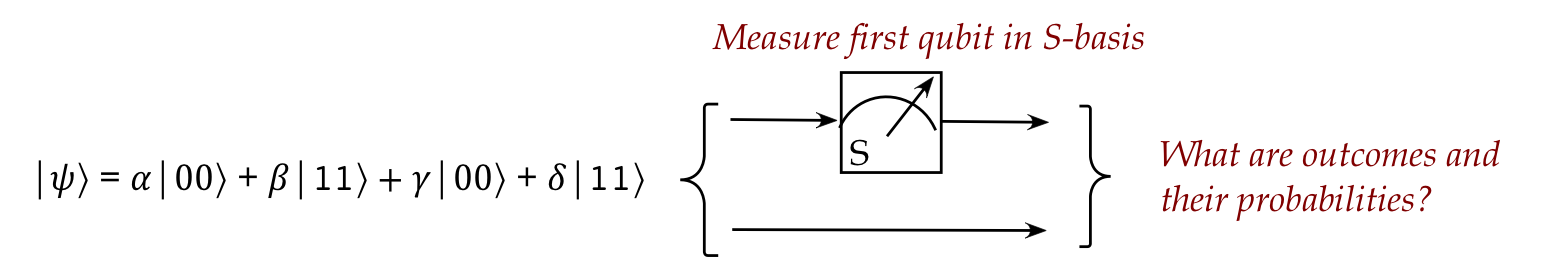
\includegraphics[width=4in]{notes/figs/n07/07measure6.png}
        \caption{Measure first qubit in H-basis}
        \label{fig:07measure6}
    \end{figure}
    
    We wish to measure the first qubit using the $\mathrm{H}$-basis $|+\rangle,|-\rangle$. The input vector is:
    
    $$
    |\psi\rangle=\frac{1}{\sqrt{2}}(|00\rangle+|11\rangle)
    $$
    
    (Recall: this is the first of the four Bell states.) Since the outcomes of the first-qubit measurement are $|+\rangle,|-\rangle$, the vector space is split into:
    
    $$
    \begin{aligned}
    &V_{1}=\operatorname{span}\{|+, 0\rangle,|+, 1\rangle\} \\
    &V_{2}=\operatorname{span}\{|-, 0\rangle,|-, 1\rangle\}
    \end{aligned}
    $$
    
    Note: We should ask: are $|+, 0\rangle,|+, 1\rangle$ orthogonal? Yes, because
    
    $$
    \langle+, 0 \mid+, 1\rangle=\langle+\mid+\rangle\langle 0 \mid 1\rangle=1 \times 0=0
    $$
    
    (The second step follows from how inner products work with tensoring.) The sets $V_{1}$ and $V_{2}$ can be written with alternative spans. For example:
    
    $$
    \begin{aligned}
    &V_{1}=\operatorname{span}\{|+,+\rangle,|+,-\rangle\} \\
    &V_{2}=\operatorname{span}\{|-,+\rangle,|-,-\rangle\}
    \end{aligned}
    $$
    
    However, we'll strive to use the standard basis where possible. Next, we'll use the constructive approach to build the projectors $P_{V_{1}}, P_{V_{2}}$ for these subspaces:
    
    $$
    \begin{aligned}
    &P_{V_{1}}=P_{+} \otimes I=|+\rangle\langle+| \otimes I \\
    &P_{V_{2}}=P_{-} \otimes I=|-\rangle\langle-| \otimes I
    \end{aligned}
    $$
    
    We might be tempted to work this out in terms of the standard basis, but let's wait until these projectors "encounter" the target vector $|\psi\rangle$. Now apply the projectors. For example, the above exercise showed that
    
    $$
    P_{V_{1}}|\psi\rangle=\frac{1}{\sqrt{2}}|+,+\rangle
    $$
    
    Which when normalized is $|+,+\rangle$. Similarly,
    
    $$
    \begin{aligned}
    P_{V_{2}}|\psi\rangle &=(1-\rangle\langle-| \otimes I) \frac{1}{\sqrt{2}}(|00\rangle+|11\rangle) \\
    &=\frac{1}{\sqrt{2}}(|-\rangle\langle-| \otimes I)(|0\rangle \otimes|0\rangle+|1\rangle \otimes|1\rangle) \\
    &=\frac{1}{\sqrt{2}}(|-\rangle\langle-\mid 0\rangle \otimes I|0\rangle+|-\rangle\langle-\mid 1\rangle \otimes I|1\rangle) \\
    &=\frac{1}{2}(|-, 0\rangle-|-, 1\rangle) \\
    &=\frac{1}{\sqrt{2}}|-\rangle \frac{1}{\sqrt{2}}(|0\rangle-|1\rangle) \\
    &=\frac{1}{\sqrt{2}}|-\rangle|-\rangle \\
    &=\frac{1}{\sqrt{2}}|-,-\rangle
    \end{aligned}
    $$
    
    (Which would get normalized as $|-,-\rangle$.) Thus, the measurement outcomes and probabilities are:
    
    $$
    \begin{aligned}
    &|+,+\rangle \quad \text { with probability } \frac{1}{2} \\
    &|-,-\rangle \quad \text { with probability } \frac{1}{2}
    \end{aligned}
    $$
    
    Note: It wasn't obvious that measuring only the first qubit would result in the second qubit becoming $|+\rangle$ or $|-\rangle$. Vith these examples, we're now in a position to outline the theoretical extension of projective measurement to multiple qubits: A measurement device corresponds to decomposition of a multi-qubit vector space $V$ into a number of orthogonal subspaces:
    
    $$
    V=V_{1} \cup \ldots \cup V_{k}
    $$
    
    This results in projectors, one per subspace: $P_{V_{i}}$. Given an input vector $|\psi\rangle \in V$, the possible outcomes of measurement are normalized versions of
    
    $$
    P_{V_{1}}|\psi\rangle, P_{V_{2}}|\psi\rangle, \ldots P_{V_{k}}|\psi\rangle
    $$
    
    That is,
    
    $$
    \frac{1}{\left.\left|P_{V_{1}}\right| \psi\right\rangle \mid} P_{V_{1}}|\psi\rangle, \frac{1}{\left.\left|P_{V_{2}}\right| \psi\right\rangle \mid} P_{V_{2}}|\psi\rangle, \ldots \frac{1}{\left.\left|P_{V_{k}}\right| \psi\right\rangle \mid} P_{V_{k}}|\psi\rangle
    $$
    
    These occur with probabilities. Outcome $\frac{1}{\left.\left|P_{V_{1}}\right| \psi\right\rangle \mid} P_{V_{1}}|\psi\rangle \quad$ with probability $\left.\left|P_{V_{1}}\right| \psi\right\rangle\left.\right|^{2}$. Outcome $\frac{1}{\left.\left|P_{V_{k}}\right| \psi\right\rangle \mid} P_{V_{k}}|\psi\rangle \quad$ with probability $\left.\left|P_{V_{k}}\right| \psi\right\rangle\left.\right|^{2}$ Note: We have not proved that this is how measurement ought to work from some underlying principle. In fact, this is a fundamental assumption, a postulate, of the theory.
    
\subsection{Projective measurement: examples}

    Let's revisit the E-91 protocol where we left out the H-basis analysis: When both Alice and Bob use the H-basis in sequence, they see the same single-qubit state: shown in Figure \ref{fig:08ekert}.
    
    \begin{figure}
        \centering
        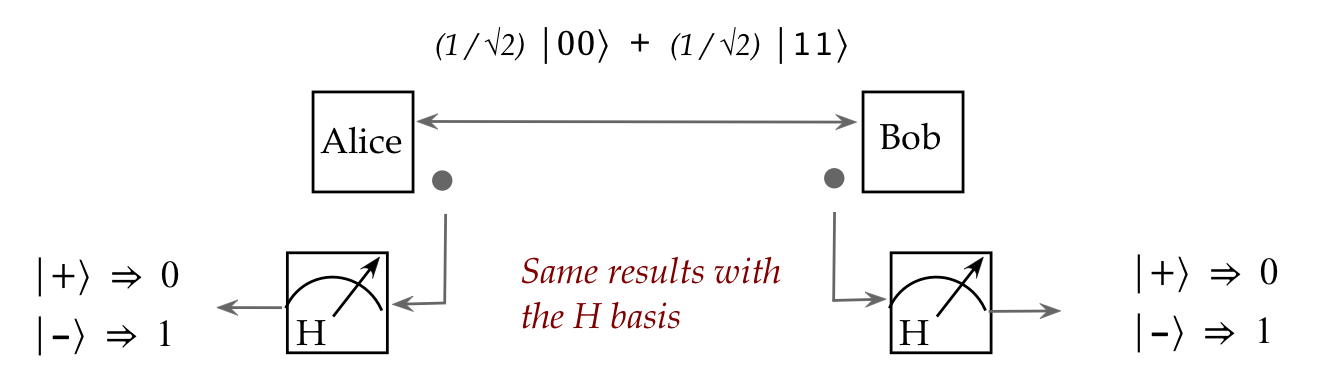
\includegraphics[width=4in]{notes/figs/n07/08ekert.png}
        \caption{Same results with the H-basis}
        \label{fig:08ekert}
    \end{figure}
    
    We already showed that when the S-basis is used in sequence, the outcomes match for both Alice and Bob. With our added theory, we can now show this for the H-basis. In the previous section, we showed that a single-qubit measurement of the entangled (Bell) state
    
    $$
    |\psi\rangle=\frac{1}{\sqrt{2}}(|00\rangle+|11\rangle)
    $$
    
    with the $\mathrm{H}$-basis resulted in outcomes
    
    $$
    \begin{aligned}
    &|+,+\rangle \quad \text { with probability } \frac{1}{2} \\
    &|-,-\rangle \quad \text { with probability } \frac{1}{2}
    \end{aligned}
    $$
    
    These are two outcomes after Alice performs her single-qubit H-basis measurement. Thus, if Alice sees $|+\rangle$ so will Bob. Likewise, if Alice sees $|-\rangle$ so will Bob. Thus, their bits match. Consider measurement with the Bell basis: Recall the Bell basis:
    
    $$
    \begin{aligned}
    &\left|\Phi^{+}\right\rangle=\frac{1}{\sqrt{2}}(|00\rangle+|11\rangle) \\
    &\left|\Phi^{-}\right\rangle=\frac{1}{\sqrt{2}}(|00\rangle-|11\rangle) \\
    &\left|\Psi^{+}\right\rangle=\frac{1}{\sqrt{2}}(|01\rangle+|10\rangle) \\
    &\left|\Psi^{-}\right\rangle=\frac{1}{\sqrt{2}}(|01\rangle-|10\rangle)
    \end{aligned}
    $$
    
    This is a 2-qubit basis. Suppose we perform a 2-qubit measurement with this basis on the general 2-qubit vector
    
    $$
    |\psi\rangle=\frac{1}{2}(\alpha|00\rangle+\beta|01\rangle+\gamma|10\rangle+\delta|11\rangle)
    $$
    
    Since we've said the measurement occurs with this basis, the four basis vectors are their own subspaces:
    
    $$
    \begin{aligned}
    &V_{\Phi^{+}}=\operatorname{span}\left\{\left|\Phi^{+}\right\rangle\right\} \\
    &V_{\Phi^{-}}=\operatorname{span}\left\{\left|\Phi^{-}\right\rangle\right\} \\
    &V_{\Psi^{+}}=\operatorname{span}\left\{\left|\Psi^{+}\right\rangle\right\} \\
    &V_{\Psi^{-}}=\operatorname{span}\left\{\left|\Psi^{-}\right\rangle\right\}
    \end{aligned}
    $$
    
    and thus, there are four projectors
    
    $$
    \left|\Phi^{+}\right\rangle\left\langle\Phi^{+}|, \quad| \Phi^{-}\right\rangle\left\langle\Phi^{-}|, \quad| \Psi^{+}\right\rangle\left\langle\Psi^{+}|, \quad| \Psi^{-}\right\rangle\left\langle\Psi^{-}\right|,
    $$
    
    Applying the first projector to the input:
    
    $$
    \begin{aligned}
    \left(\left|\Phi^{+}\right\rangle\left\langle\Phi^{+}\right|\right)|\psi\rangle &=\left|\Phi^{+}\right\rangle\left\langle\Phi^{+} \mid \psi\right\rangle \\
    &\left.=\frac{1}{2}\left|\Phi^{+}\right\rangle\left\langle\Phi^{+}|\alpha| 00\right\rangle+\beta|01\rangle+\gamma|10\rangle+\delta|11\rangle\right\rangle \\
    &=\frac{1}{2}\left|\Phi^{+}\right\rangle\left(\alpha\left\langle\Phi^{+} \mid 00\right\rangle+\beta\left\langle\Phi^{+} \mid 01\right\rangle+\gamma\left\langle\Phi^{+} \mid 10\right\rangle+\delta\left\langle\Phi^{+} \mid 11\right\rangle\right) \\
    &=\frac{\alpha+\delta}{2 \sqrt{2}}\left|\Phi^{+}\right\rangle
    \end{aligned}
    $$
    
    Similarly,
    
    $$
    \begin{aligned}
    &\left(\left|\Phi^{-}\right\rangle\left\langle\Phi^{-}\right|\right)|\psi\rangle=\frac{\alpha-\delta}{2 \sqrt{2}}\left|\Phi^{-}\right\rangle \\
    &\left(\left|\Psi^{+}\right\rangle\left\langle\Psi^{+}\right|\right)|\psi\rangle=\frac{\beta+\gamma}{2 \sqrt{2}}\left|\Psi^{+}\right\rangle \\
    &\left(\left|\Psi^{-}\right\rangle\left\langle\Psi^{-}\right|\right)|\psi\rangle=\frac{\beta-\gamma}{2 \sqrt{2}}\left|\Psi^{-}\right\rangle
    \end{aligned}
    $$
    
    Thus, the outcomes are the Bell vectors with probabilities
    
    $$
    \begin{array}{lc}
    \left|\Phi^{+}\right\rangle & \text {with probability }\left|\frac{\alpha+\delta}{2 \sqrt{2}}\right|^{2} \\
    \left|\Phi^{-}\right\rangle & \text {with probability }\left|\frac{\alpha-\delta}{2 \sqrt{2}}\right|^{2} \\
    \left|\Psi^{+}\right\rangle & \text {with probability }\left|\frac{\beta+\gamma}{2 \sqrt{2}}\right|^{2} \\
    \left|\Psi^{-}\right\rangle & \text {with probability }\left|\frac{\beta-\gamma}{2 \sqrt{2}}\right|^{2}
    \end{array}
    $$

    Note: This example is merely of theoretical interest. Just because we dream up a measurement basis does not mean it can be physically implemented with an actual device. A hypothetical 3-qubit example: Suppose there was a way to test whether two qubits are equal. And suppose we apply this to the first and third qubits of a 3-qubit system. Then, such a measurement will divide the space into two subspaces:
    
    $$
    \begin{aligned}
    &V_{1}=\operatorname{span}\{|000\rangle,|010\rangle,|101\rangle,|111\rangle\} \\
    &V_{2}=\operatorname{span}\{|001\rangle,|011\rangle,|100\rangle,|110\rangle\}
    \end{aligned}
    $$
    
    Note: the vectors spanning $V_{1}$ have their first and third bits equal. The projectors are:
    
    $$
    \begin{aligned}
    &P_{V_{1}}=|000\rangle\langle 000|+| 010\rangle\langle 010|+| 101\rangle\langle 101|+| 111\rangle\langle 111| \\
    &P_{V_{2}}=|001\rangle\langle 001|+| 011\rangle\langle 011|+| 100\rangle\langle 100|+| 110\rangle\langle 110|
    \end{aligned}
    $$
    
    One can then apply these to an input vector $|\psi\rangle$ in the usual way. For example, suppose
    
    $$
    |\psi\rangle=\frac{1}{\sqrt{3}}(|000\rangle+|001\rangle+|010\rangle)
    $$
    
    Then
    
    $$
    \begin{aligned}
    &P_{V_{1}}|\psi\rangle=\frac{1}{\sqrt{3}}(|000\rangle \\
    &P_{V_{2}}|\psi\rangle=\frac{1}{\sqrt{3}}|001\rangle
    \end{aligned}
    $$
    
    Thus, the outcomes and probabilities are:
    
    $$
    \begin{array}{rr}
    \frac{1}{\sqrt{2}}(|000\rangle+|010\rangle) & \text { with probability } \frac{2}{3} \\
    |001\rangle & \text { with probability } \frac{1}{3}
    \end{array}
    $$

\subsection{Projective measurement in stages}

    Consider measurements in sequence, as in this example in Figure \ref{fig:09measure8}.
    
    \begin{figure}
        \centering
        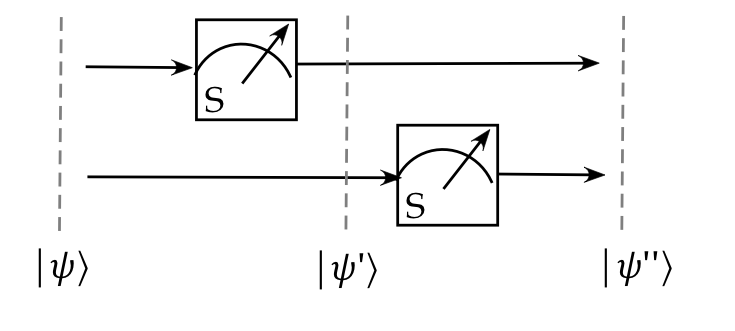
\includegraphics[width=4in]{notes/figs/n07/09measure8.png}
        \caption{Measurements in Sequence}
        \label{fig:09measure8}
    \end{figure}
    
    Here, the input is a 2 -qubit state $|\psi\rangle$. Then, the top qubit is first measured, which results in some state $\left|\psi^{\prime}\right\rangle$. After this, the vector is measured in the second qubit, which leaves the state $\left|\psi^{\prime \prime}\right\rangle$. The question arises: is there a single 2 -qubit measurement that is equivalent to the sequence of 1 -qubit measurements? Let's analyze the above scenario: Suppose the input $|\psi\rangle$ is the generic 2-qubit state
    
    $$
    |\psi\rangle=(\alpha|00\rangle+\beta|01\rangle+\gamma|10\rangle+\delta|11\rangle)
    $$
    
    Now, the projectors for the first measurement are:
    
    $$
    \begin{aligned}
    &P_{0}=|0\rangle\langle 0|\otimes I=| 00\rangle\langle 00|+| 01\rangle\langle 01| \\
    &P_{1}=|1\rangle\langle 1|\otimes I=| 10\rangle\langle 10|+| 11\rangle\langle 11|
    \end{aligned}
    $$
    
    From which,
    
    $$
    \begin{aligned}
    &P_{0}|\psi\rangle=\alpha|00\rangle+\beta|01\rangle \\
    &P_{1}|\psi\rangle=\gamma|10\rangle+\delta|11\rangle
    \end{aligned}
    $$
    
    which we'll normalize and name:
    
    $$
    \begin{aligned}
    \left|\psi_{0}\right\rangle &=\frac{1}{\left.\left|P_{0}\right| \psi\right\rangle \mid} P_{0}|\psi\rangle=\frac{1}{\sqrt{|\alpha|^{2}+|\beta|^{2}}}(\alpha|00\rangle+\beta|01\rangle) \\
    \left|\psi_{1}\right\rangle &=\frac{1}{\left.\left|P_{1}\right| \psi\right\rangle \mid} P_{1}|\psi\rangle=\frac{1}{\sqrt{|\gamma|^{2}+|\delta|^{2}}}(\gamma|10\rangle+\delta|11\rangle)
    \end{aligned}
    $$
    
    Next, each of these outcomes occur with the following probabilities:
    
    $$
    \begin{array}{ll}
    \left|\psi_{0}\right\rangle & \text { occurs with probability } \left.\left|P_{0}\right| \psi\right\rangle\left.\right|^{2}=|\alpha|^{2}+|\beta|^{2} \\
    \left|\psi_{1}\right\rangle & \text { occurs with probability } \left.\left|P_{1}\right| \psi\right\rangle\left.\right|^{2}=|\gamma|^{2}+|\delta|^{2}
    \end{array}
    $$
    
    Now for a given measurement, either one (but not both) will be an input into the second measurement. We'll consider both cases. The projectors for the second measurement are:
    
    $$
    \begin{aligned}
    &P_{2}=I \otimes|0\rangle\langle 0|=| 00\rangle\langle 00|+| 10\rangle\langle 10| \\
    &P_{3}=I \otimes|1\rangle\langle 1|=| 01\rangle\langle 01|+| 11\rangle\langle 11|
    \end{aligned}
    $$
    
    We will next apply these projectors to the possible outcomes, $\left|\psi_{0}\right\rangle$ and $\left|\psi_{1}\right\rangle$, from the first stage:
    
    $$
    \begin{aligned}
    &P_{2}\left|\psi_{0}\right\rangle=(|00\rangle\langle 00|+| 10\rangle\langle 10|) \frac{\alpha}{\sqrt{|\alpha|^{2}+|\beta|^{2}}}(\alpha|00\rangle+\beta|01\rangle)=\frac{\alpha}{\sqrt{|\alpha|^{2}+|\beta|^{2}}}|00\rangle \\
    &P_{2}\left|\psi_{1}\right\rangle=(|00\rangle\langle 00|+| 10\rangle\langle 10|) \frac{\gamma}{\sqrt{|y|^{2}+|\delta|^{2}}}(\gamma|10\rangle+\delta|11\rangle)=\frac{\gamma}{\sqrt{|\gamma|^{2}+|\delta|^{2}}}|10\rangle \\
    &P_{3}\left|\psi_{0}\right\rangle=(|01\rangle\langle 01|+| 11\rangle\langle 11|) \frac{\beta}{\sqrt{|\alpha|^{2}+|\beta|^{2}}}(\alpha|00\rangle+\beta|01\rangle)=\frac{\beta}{\sqrt{|\alpha|^{2}+|\beta|^{2}}}|01\rangle \\
    &P_{3}\left|\psi_{1}\right\rangle=(|01\rangle\langle 01|+| 11\rangle\langle 11|) \frac{\delta}{\sqrt{|\gamma|^{2}+|\delta|^{2}}}(\gamma|10\rangle+\delta|11\rangle)=\frac{\delta}{\sqrt{|\gamma|^{2}+|\delta|^{2}}}|11\rangle
    \end{aligned}
    $$
    
    Observe that the outcomes (normalized) are the standard 2-qubit vectors: $|00\rangle,|01\rangle,|10\rangle,|11\rangle$. These occur with probabilities
    
    $$
    \begin{aligned}
    |00\rangle \text { occurs with probability } |\alpha|^{2}\\
    |01\rangle \text{ occurs with probability } |\rho|^{2}\\
    |10\rangle \text{ occurs with probability } |\gamma|^{2}\\
    |11\rangle \text{ occurs with probability } |\delta|^{2}
    \end{aligned}
    $$
    
    (See exercise below to fill in one step: how did terms like $\sqrt{|\alpha|^{2}+|\beta|^{2}}$ and $\sqrt{|\gamma|^{2}+|\delta|^{2}}$ disappear?). But these are exactly the outcomes and probabilities one gets with 2 -qubit measurement in the standard basis! That is, with projectors
    
    $$
    \begin{aligned}
    &Q_{0}=|00\rangle\langle 00| \\
    &Q_{1}=|01\rangle\langle 01| \\
    &Q_{2}=|10\rangle\langle 10| \\
    &Q_{3}=|11\rangle\langle 11|
    \end{aligned}
    $$
    
    applied to
    
    $$
    |\psi\rangle=(\alpha|00\rangle+\beta|01\rangle+\gamma|10\rangle+\delta|11\rangle)
    $$
    
    one gets the same outcomes with the same probabilities. Thus, we've answered the question: what 2 -qubit measurement corresponds to the sequence of 1 -qubit measurements from earlier?
    
    Combining projectors in sequenced measurements: We went through a lot of trouble in applying the two sets of projectors in sequence above. Let's ask: could we have applied the projectors in sequence and then normalize? The answer is: yes! (And the algebra is much simpler) Recall that we started with input vector $|\psi\rangle$. Then we applied the first stage:
    
    $$
    \begin{aligned}
    &P_{0}|\psi\rangle=(|0\rangle\langle 0| \otimes I)|\psi\rangle \\
    &P_{1}|\psi\rangle=(|1\rangle\langle 1| \otimes I)|\psi\rangle
    \end{aligned}
    $$
    
    Now consider applying the second stage directly, without normalizing:
    
    $$
    \begin{aligned}
    &P_{2} P_{0}|\psi\rangle=(I \otimes|0\rangle\langle 0|)(|0\rangle\langle 0| \otimes I)|\psi\rangle \\
    &P_{2} P_{1}|\psi\rangle=(I \otimes|0\rangle\langle 0|)(|1\rangle\langle 1| \otimes I)|\psi\rangle \\
    &P_{3} P_{0}|\psi\rangle=(I \otimes|1\rangle\langle 1|)(|0\rangle\langle 0| \otimes I)|\psi\rangle \\
    &P_{3} P_{1}|\psi\rangle=(I \otimes|1\rangle\langle 1|)(|1\rangle\langle 1| \otimes I)|\psi\rangle
    \end{aligned}
    $$
    
    Now use the rules for tensors of matrices: $(A \otimes B)(C \otimes D)=(A B \otimes C D)$. Applying, we see that
    
    $$
    \begin{aligned}
    P_{2} P_{0}|\psi\rangle &=(|0\rangle\langle 0|\otimes| 0\rangle\langle 0|)|\psi\rangle=|00\rangle\langle 00|| \psi\rangle \\
    P_{2} P_{1}|\psi\rangle &=(|1\rangle\langle 1|\otimes| 0\rangle\langle 0|)|\psi\rangle=|10\rangle\langle 10|| \psi\rangle \\
    P_{3} P_{0}|\psi\rangle &=(|0\rangle\langle 0|\otimes| 1\rangle\langle 1|)|\psi\rangle=|01\rangle\langle 01|| \psi\rangle \\
    P_{3} P_{1}|\psi\rangle &=(|1\rangle\langle 1|\otimes| 1\rangle\langle 1|)|\psi\rangle=|11\rangle\langle 11|| \psi\rangle
    \end{aligned}
    $$
    
    These are just the standard-basis 2-qubit projectors. There is an important practical implication: Physically implementing a 2-qubit measurement is difficult. What we've seen is that a 2-qubit standard-basis measurement can be done in two stages of standard-basis 1 -qubit measurements. This is what happens in practice.

\subsection{Unitary actions in sequence and across qubits}

    We of course want to "do things" to qubits before measuring. The only way to change qubits without measuring is to apply a unitary operation. Let's highlight a few general aspects to applying unitary operations: Consider this 2-qubit example shown in Figure \ref{fig:09measure8}.
    
    \begin{figure}
        \centering
        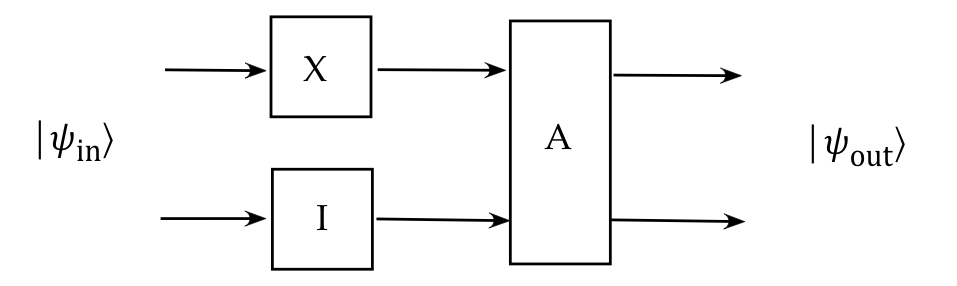
\includegraphics[width=4in]{notes/figs/n07/10unitary1.png}
        \caption{2-qubit example}
        \label{fig:09measure8}
    \end{figure}
    
    $X$ and $I$ are 1-qubit unitary operators. A is a 2-qubit operator. We want to know: what is the output vector as a result of applying these operators to the input vector? Our diagramming uses the "flying qubit" paradigm to imagine a multi-qubit vector going from left to right through the unitary operators. Thus, we will be interested in the multi-qubit state at each stage shown in Figure \ref{fig:11unitary2}.

    \begin{figure}
        \centering
        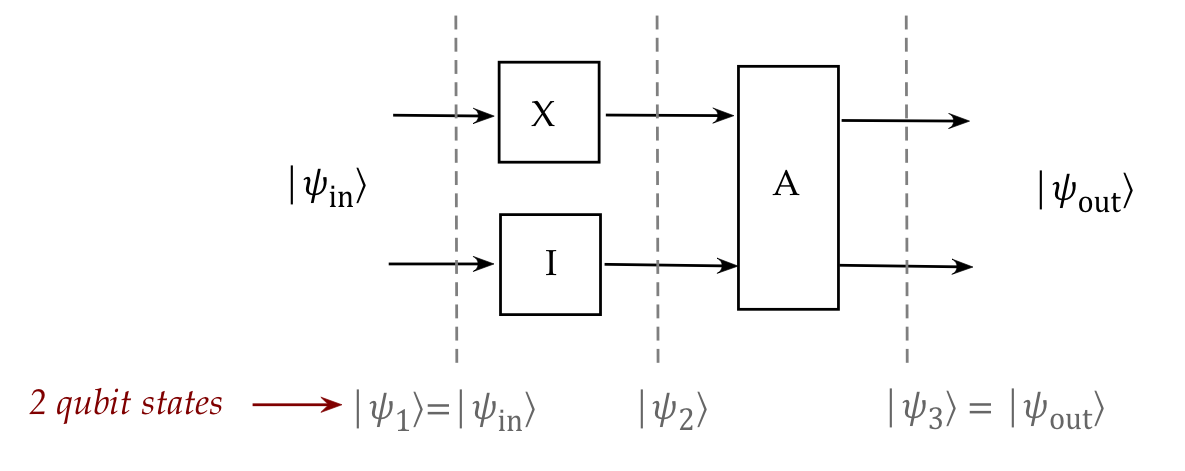
\includegraphics[width=4in]{notes/figs/n07/11unitary2.png}
        \caption{2-qubit states}
        \label{fig:11unitary2}
    \end{figure}

    Think of the dashed lines representing stages in the time-evolution of this system. Thus, initial 2-qubit state is $\left|\psi_{1}\right\rangle$. After the application of $X$ to the first qubit, and no change $I$ to the second, the 2 -qubit state is now $\left|\psi_{2}\right\rangle$. We've seen that this corresponds to the unitary operator
    
    $$
    X \otimes I=\left[\begin{array}{ll}
    0 & 1 \\
    1 & 0
    \end{array}\right] \otimes I=\left[\begin{array}{ll}
    0 & I \\
    I & 0
    \end{array}\right]=\left[\begin{array}{llll}
    0 & 0 & 1 & 0 \\
    0 & 0 & 0 & 1 \\
    1 & 0 & 0 & 0 \\
    0 & 1 & 0 & 0
    \end{array}\right]
    $$
    
    After applying the operator $A$ the result is $\left|\psi_{3}\right\rangle$. Here, we're going to use
    
    $$
    A=\left[\begin{array}{llll}
    0 & 0 & 0 & 1 \\
    0 & 0 & 1 & 0 \\
    0 & 1 & 0 & 0 \\
    1 & 0 & 0 & 0
    \end{array}\right]
    $$
    
    At every stage a complete 2-qubit unitary operation applies as shown in Figure \ref{fig:11unitary2}.
    
    \begin{figure}
        \centering
        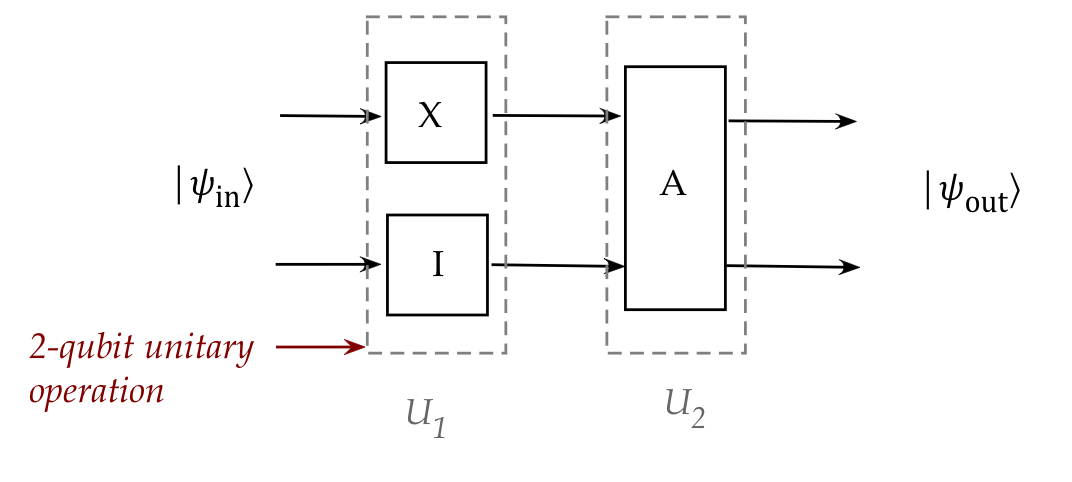
\includegraphics[width=4in]{notes/figs/n07/12unitary3.png}
        \caption{2-qubit unitary operator}
        \label{fig:12unitary3}
    \end{figure}

    Even though nothing is done to the second qubit, we write that as the "do nothing" operator $I$. We could (and will often) draw Figure \ref{fig:13unitary4}.
    
    \begin{figure}
        \centering
        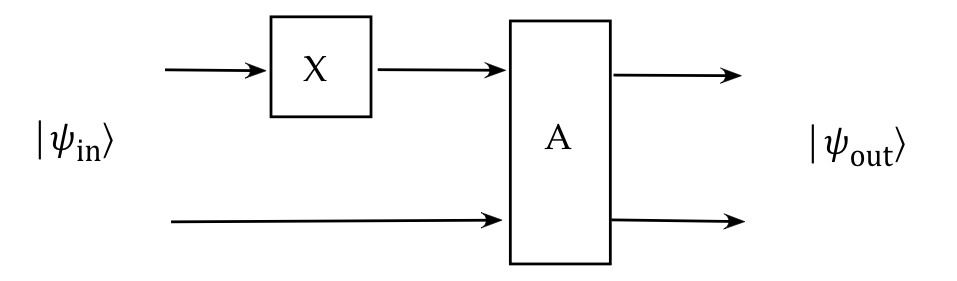
\includegraphics[width=4in]{notes/figs/n07/13unitary4.png}
        \caption{Simplification with obscured first stage}
        \label{fig:13unitary4}
    \end{figure}
    
    But this obscures the fact that the first stage is really the 2 -qubit operator $X \otimes I$. These aspects become more clear algebraically: Suppose the input 2 -qubit vector is $|\psi\rangle$. The first stage produces
    
    $$
    \left|\psi_{2}\right\rangle=(X \otimes I)|\psi\rangle
    $$
    
    And this is acted on by the second stage:

    $$
    \left|\psi_{3}\right\rangle=A\left|\psi_{2}\right\rangle
    $$
    
    Which we can combine as:
    
    $$
    \left|\psi_{3}\right\rangle=A(X \otimes I)|\psi\rangle
    $$
    
    Let's emphasize the matrix dimensions:
    
    $$
    \left|\psi_{3}\right\rangle_{4 \times 1}=A_{4 \times 4}\left(X_{2 \times 2} \otimes I_{2 \times 2}\right)|\psi\rangle_{4 \times 1}
    $$
    
    Thus, we could not write
    
    $$
    \left|\psi_{3}\right\rangle=A X|\psi\rangle \quad \text { Incorrect! }
    $$
    
    Continuing with the example: Suppose the operator $A$ happens to be $A=X \otimes X$. Then the two stages can be tensored as:
    
    $$
    \begin{aligned}
    A(X \otimes I) &=(X \otimes X)(X \otimes I) & & \text { Sub for } A \\
    &=(X X \otimes X I) & & \text { Tensor bilinearity } \\
    &=(I \otimes X) & & \text { Shown in exercise }
    \end{aligned}
    $$
    
    Now let's apply this to the generic 2-qubit vector
    
    $$
    |\psi\rangle=\alpha|00\rangle+\beta|01\rangle+\gamma|10\rangle+\delta|11\rangle
    $$
    
    In Dirac form
    
    $$
    \begin{aligned}
    I \otimes X &=(|0\rangle\langle 0|+| 1\rangle\langle 1|) \otimes(|0\rangle\langle 1|+| 1\rangle\langle 0|) & \text { Dirac versions of the } 1 \text {-qubit ops } \\
    &=(|0\rangle\langle 0|\otimes| 0\rangle\langle 1|)+(|0\rangle\langle 0|\otimes| 1\rangle\langle 0|)+(|1\rangle\langle 1|\otimes| 0\rangle\langle 1|)+(|1\rangle\langle 1|\otimes| 1\rangle\langle 0|) & \text { Distribution over + } \\
    &=|00\rangle\langle 01|+| 01\rangle\langle 00|+| 10\rangle\langle 11|+| 11\rangle\langle 10| & \text { Tenser rules for outer-products }
    \end{aligned}
    $$
    
    Thus,
    
    $$
    \begin{aligned}
    (I \otimes X)|\psi\rangle &=(|00\rangle\langle 01|+| 01\rangle\langle 00|+| 10\rangle\langle 11|+| 11\rangle\langle 10|) \alpha|00\rangle+\beta|01\rangle+\gamma|10\rangle+\delta|11\rangle \\
    &=\beta|00\rangle+\alpha|01\rangle+\delta|10\rangle+\gamma|11\rangle
    \end{aligned}
    $$
    
    Let's now generalize these ideas to the $\mathrm{n}$-qubit case: A single-qubit unitary operation $A_{k}$ performed on the $k$-th qubit corresponds to the $n$-qubit unitary operation
    
    $$
    I \otimes I \otimes \ldots \otimes A_{k} \otimes \ldots \otimes I
    $$
    
    When a sequence of n-qubit operations are applied: The diagram goes left to right. But the matrices go right to left:
    
    $$
    U_{m} U_{m-1} \ldots U_{2} U_{1}|\psi\rangle
    $$
    
    That is, $U_{1}$ is first applied, then $U_{2}$ etc. A collection of multi-qubit operators can be applied at any stage, for example as shown in Figure \ref{fig:14unitary5}.
    
    \begin{figure}
        \centering
        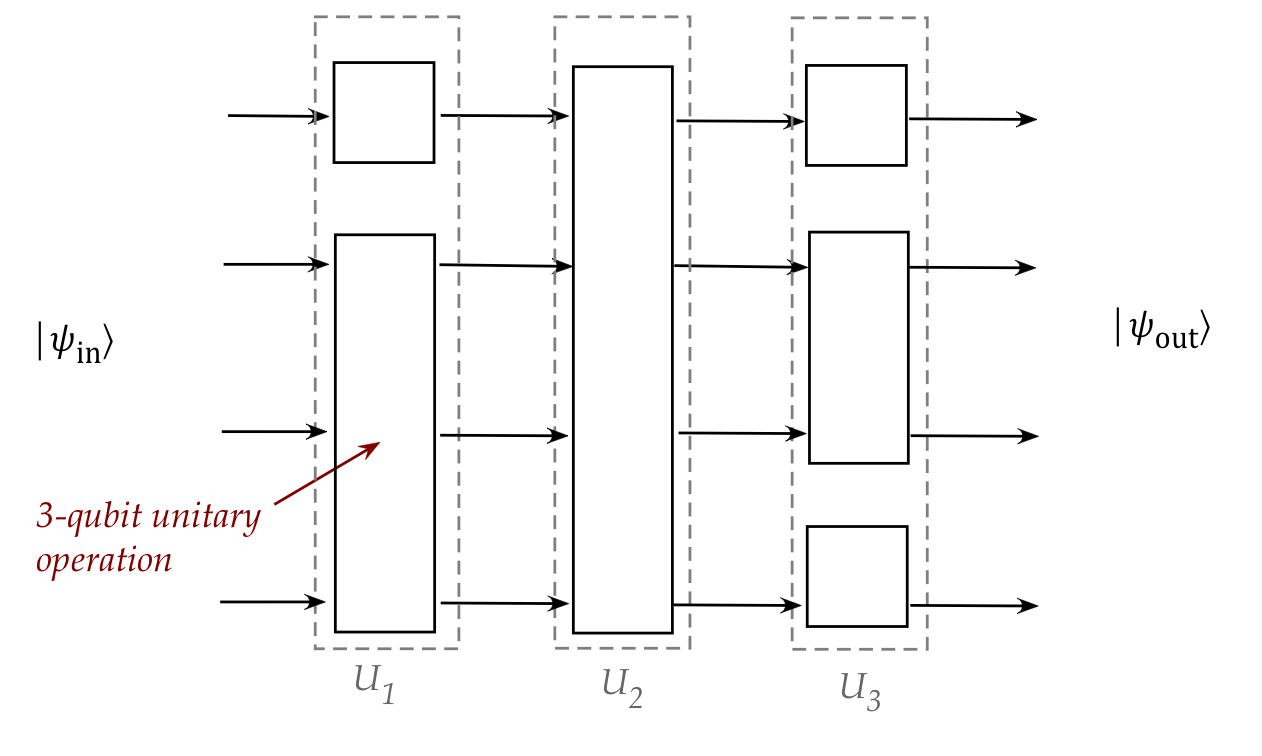
\includegraphics[width=4in]{notes/figs/n07/14unitary5.png}
        \caption{3-qubit unitary operation}
        \label{fig:14unitary5}
    \end{figure}
    
    Here: Think of tensoring applying vertically. The first stage, for example, is a tensor of 1 -qubit unitary with a 3 -qubit unitary. And regular operator products applied horizontally: $U_{m} U_{m-1} \ldots U_{2} U_{1}$. The theory developed earlier showed that: Tensored unitary operators (going vertically) are unitary. Products of unitary operators (going horizontally) are unitary. The big implication: Quantum computations can be created by designing unitary operations in sequence, each of which is composed (vertically) of smaller operations. Where does measurement fit in? The answer: anywhere! Reference Figure \ref{fig:15unitary6}.
    
    \begin{figure}
        \centering
        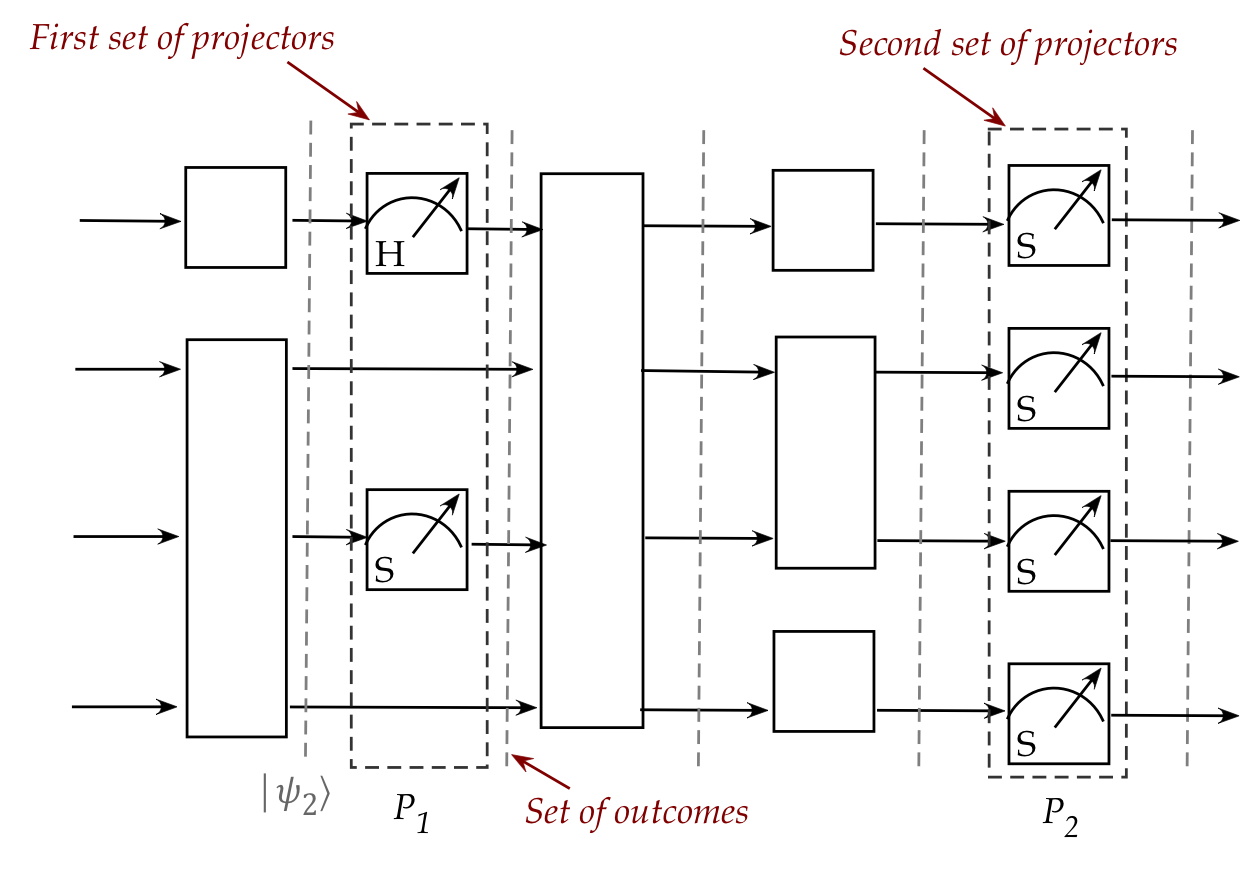
\includegraphics[width=4in]{notes/figs/n07/15unitary6.png}
        \caption{first and second set of projectors}
        \label{fig:15unitary6}
    \end{figure}
    
    When a measurement occurs, it is represented by a set of projectors (for each basis vector of the measuring device). We cannot apply a single projector. After the first measurement, the outcomes are probabilistic and cannot be represented by a single state. Typically, all measurements occur after the last unitary operation shown in Figure \ref{fig:16unitary7}.
    
    \begin{figure}
        \centering
        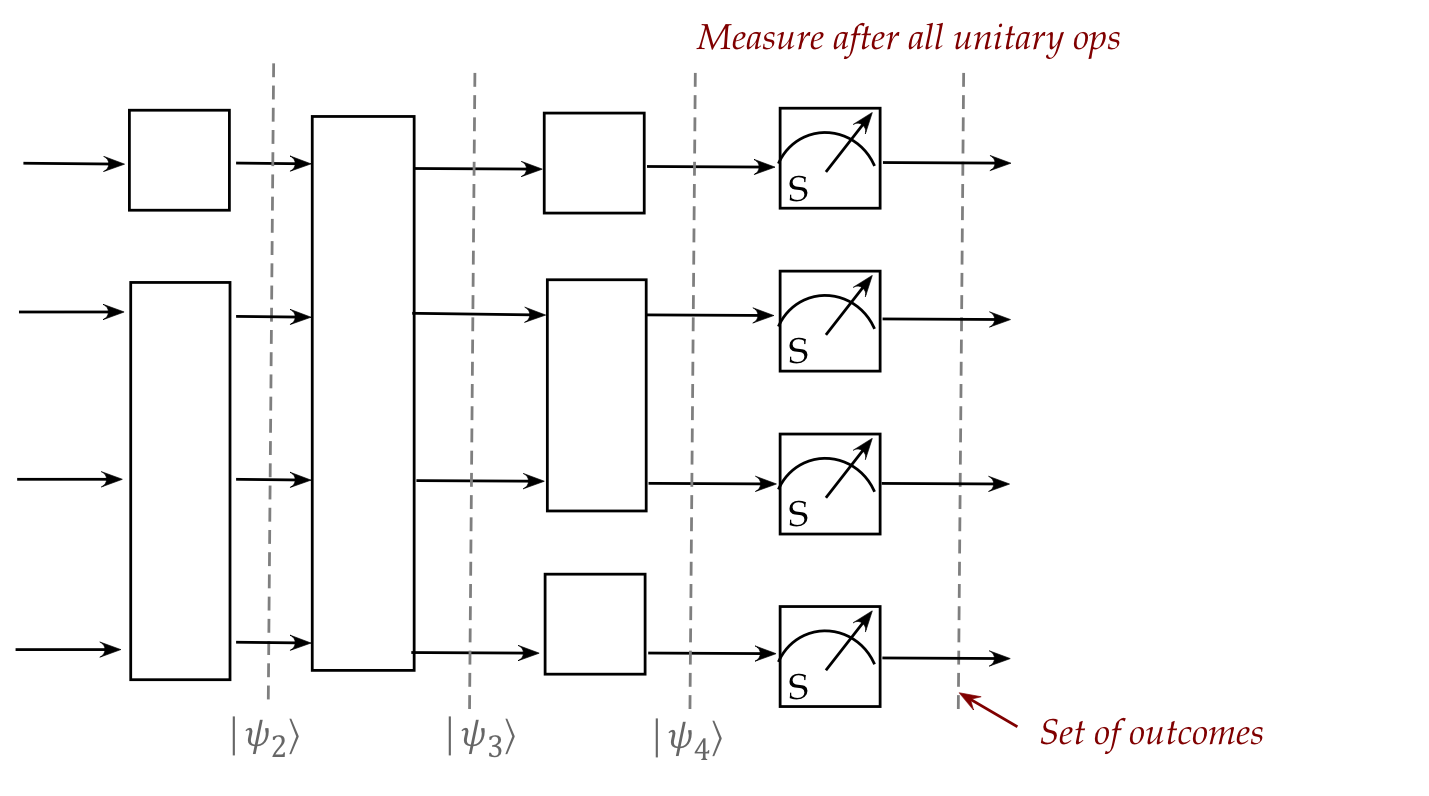
\includegraphics[width=4in]{notes/figs/n07/16unitary7.png}
        \caption{measure after all unitary ops}
        \label{fig:16unitary7}
    \end{figure}
    
    This is easier to analyze. The basis is most often the standard basis. This unitary-followed-by-measurement is called the standard circuit model. The task of developing a quantum computation is now clear in this framework shown in Figure \ref{fig:17unitary8}.
    
    \begin{figure}
        \centering
        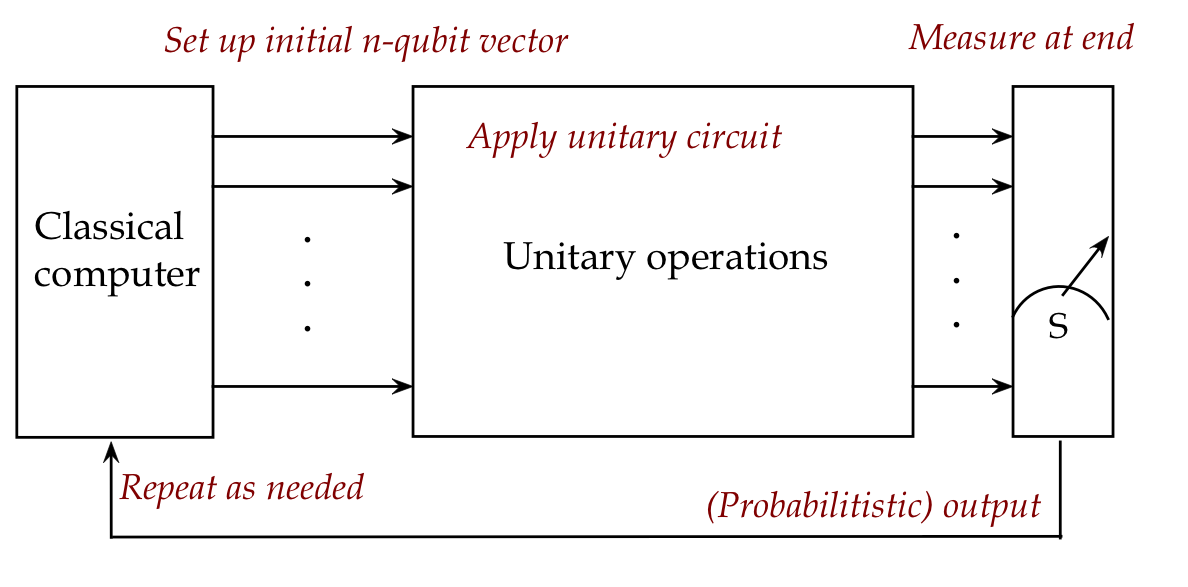
\includegraphics[width=4in]{notes/figs/n07/17unitary8.png}
        \caption{Quantum computation framework}
        \label{fig:17unitary8}
    \end{figure}
    
    Figure out the unitary operations and assemble them into a circuit. Analyse the results of measurement to infer the outcomes. Repeat as needed. What remains for us: What unitary operations are useful (and practical to implement)? How does one systematically construct a circuit? How do circuits lead to useful algorithms? How can we exploit quantum parallelism? Let's explore the last point: You might have noticed a problem with the classical-quantum looped architecture above: If a classical computer sets up an initial n-qubit vector like $|00 \ldots 0\rangle$, why not just have the classical computer simulate the circuit? The advantage: no randomness! However, consider this 2 -qubit input state:
    
    $$
    |\psi\rangle=\frac{1}{2}(|00\rangle+|01\rangle+|10\rangle+|11\rangle)
    $$
    
    Note: All four 2-qubit basis vectors are "in there". We might hope that a circuit acting on $|\psi\rangle$ somehow does something to each basis vector at the same time. For 3 qubits, the equivalent state that combines all basis vectors with equal weight is:
    
    $$
    |\psi\rangle=\frac{1}{\sqrt{8}}(|000\rangle+|001\rangle+|010\rangle+|011\rangle+|100\rangle+|101\rangle+|110\rangle+|111\rangle)
    $$
    
    If measured, the probability of seeing any one of them is the same: $\left(\frac{1}{\sqrt{8}}\right)^{2}=\frac{1}{8}$ We can extend this to n-qubits with the state:
    
    $$
    |\psi\rangle=\frac{1}{\sqrt{2^{n}}}(|00 \ldots 0\rangle+\ldots+|11 \ldots 1\rangle)
    $$
    
    Terminology: superposition. The term superposition simply refers to a linear combination. The above examples are sometimes called equal-superposition states for the standard basis. An equal-superposition state is often the starting state for many quantum algorithms. The potential for speed up or parallelism: If a circuit acts on the equal-superposition state, it can act on all $2^{n}$ states at the same time. This has the potential of providing exponential speed up over classical machines. However, measurement can "ruin" this potential because the outcomes are probabilistic, and because it forces the state into one of the $2^{n}$ basis vectors. Precisely explaining quantum speed-up remains an unresolved issue: Some results show that entanglement must be present when speed-up occurs. Other results show speed up without exploiting superposition.
    
\subsection{The Hadamard operator}

    The Hadamard operator is one of the most important operators in quantum computing: It is frequently used to create the $\mathrm{n}$-qubit equal-superposition as the input vector for a computation. It also features in intermediate computations, sometimes just on one qubit. To see where it comes from, we'll start with the 1-qubit idea of transforming $|0\rangle$ into the 1-qubit equal-superposition
    
    $$
    |+\rangle=\frac{1}{\sqrt{2}}|0\rangle+\frac{1}{\sqrt{2}}|1\rangle
    $$
    
    Suppose there is some unitary operator $H$ such that
    
    $$
    H|0\rangle=\frac{1}{\sqrt{2}}|0\rangle+\frac{1}{\sqrt{2}}|1\rangle
    $$
    
    In matrix form, this unknown operator could be represented by four numbers
    
    $$
    \left[\begin{array}{ll}
    a & b \\
    c & d
    \end{array}\right]\left[\begin{array}{l}
    1 \\
    0
    \end{array}\right]=\frac{1}{\sqrt{2}}|0\rangle+\frac{1}{\sqrt{2}}|1\rangle
    $$
    
    or
    
    $$
    \left[\begin{array}{l}
    a \\
    c
    \end{array}\right]=\left[\begin{array}{c}
    \frac{1}{\sqrt{2}} \\
    \frac{1}{\sqrt{2}}
    \end{array}\right]
    $$
    
    Since the rows are orthonormal, we must have
    
    $$
    \begin{aligned}
    &|a|^{2}+|b|^{2}=1 \\
    &|c|^{2}+|d|^{2}=1
    \end{aligned}
    $$
    
    or
    
    $$
    \begin{aligned}
    &|b|^{2}=1-|a|^{2}=1-\left(\frac{1}{\sqrt{2}}\right)=\frac{1}{2} \\
    &|d|^{2}=1-|c|^{2}=1-\left(\frac{1}{\sqrt{2}}\right)=\frac{1}{2}
    \end{aligned}
    $$
    
    Thus,
    
    $$
    \begin{aligned}
    &b=\pm \frac{1}{\sqrt{2}} \\
    &d=\pm \frac{1}{\sqrt{2}}
    \end{aligned}
    $$
    
    However: $b$ and $d$ cannot have the same sign. For example
    
    $$
    \left[\begin{array}{ll}
    \frac{1}{\sqrt{2}} & \frac{1}{\sqrt{2}} \\
    \frac{1}{\sqrt{2}} & \frac{1}{\sqrt{2}}
    \end{array}\right]
    $$
    
    would not work because the two columns are not orthogonal. But either of
    
    $$
    \left[\begin{array}{cc}
    \frac{1}{\sqrt{2}} & \frac{1}{\sqrt{2}} \\
    \frac{1}{\sqrt{2}} & -\frac{1}{\sqrt{2}}
    \end{array}\right] \quad \text { or } \quad\left[\begin{array}{cc}
    \frac{1}{\sqrt{2}} & -\frac{1}{\sqrt{2}} \\
    \frac{1}{\sqrt{2}} & \frac{1}{\sqrt{2}}
    \end{array}\right]
    $$
    
    would work. The former is the $H$ operator and gives us the definition of $|-\rangle$ :
    
    $$
    H|1\rangle=\left[\begin{array}{cc}
    \frac{1}{\sqrt{2}} & \frac{1}{\sqrt{2}} \\
    \frac{1}{\sqrt{2}} & -\frac{1}{\sqrt{2}}
    \end{array}\right]\left[\begin{array}{l}
    0 \\
    1
    \end{array}\right]=\left[\begin{array}{c}
    \frac{1}{\sqrt{2}} \\
    -\frac{1}{\sqrt{2}}
    \end{array}\right]=|-\rangle
    $$
    
    Thus, in the 1-qubit case, the Hadamard operator $H$ creates equal-superposition:
    
    $$
    H|0\rangle=\frac{1}{\sqrt{2}}|0\rangle+\frac{1}{\sqrt{2}}|1\rangle
    $$
    
    Terminology: $H$ is also called the Walsh-Hadamard transform. Next consider equal superposition in 2 qubits: The vector in this case is:
    
    $$
    |\psi\rangle=\frac{1}{2}|00\rangle+\frac{1}{2}|01\rangle+\frac{1}{2}|10\rangle+\frac{1}{2}|11\rangle
    $$
    
    We now seek a 2 -qubit unitary operator to transform $|00\rangle$ into $|\psi\rangle$:
    
    $$
    A|00\rangle=\frac{1}{2}|00\rangle+\frac{1}{2}|01\rangle+\frac{1}{2}|10\rangle+\frac{1}{2}|11\rangle
    $$
    
    Observe that
    
    $$
    |+\rangle|+\rangle=|+\rangle \otimes|+\rangle=\frac{1}{\sqrt{2}}(|0\rangle+|1\rangle) \otimes \frac{1}{\sqrt{2}}(|0\rangle+|1\rangle)=\frac{1}{2}|00\rangle+\frac{1}{2}|01\rangle+\frac{1}{2}|10\rangle+\frac{1}{2}|11\rangle
    $$
    
    So, clearly the desired operator $A$ will satisfy
    
    $$
    A|00\rangle=|+\rangle \otimes|+\rangle
    $$
    
    or
    
    $$
    A(|0\rangle \otimes|0\rangle)=|+\rangle \otimes|+\rangle
    $$
    
    But we showed in the 1-qubit case that $H|0\rangle=|+\rangle$. Substituting
    
    $$
    |+\rangle \otimes|+\rangle=H|0\rangle \otimes H|0\rangle=(H \otimes H)(|0\rangle \otimes|0\rangle)
    $$
    
    which means we've found our operator
    
    $$
    A=H \otimes H
    $$
    
    And because tensor products preserve unitarity, $H \otimes H$ is unitary. The n-qubit version: The $\mathrm{n}$-qubit equal-superposition merely tensors $|+\rangle$ qubits:
    
    $$
    |+\rangle|+\rangle \ldots|+\rangle=\left(\frac{1}{\sqrt{2}}|0\rangle+\frac{1}{\sqrt{2}}|1\rangle\right) \otimes\left(\frac{1}{\sqrt{2}}|0\rangle+\frac{1}{\sqrt{2}}|1\rangle\right) \otimes \ldots \otimes\left(\frac{1}{\sqrt{2}}|0\rangle+\frac{1}{\sqrt{2}}|1\rangle\right)=\left(\frac{1}{\sqrt{2}}\right)^{n}(|00 \ldots 0\rangle+|00 \ldots 1\rangle+\ldots+|11 \ldots 1\rangle)
    $$
    
    Which means the transform needed to convert $|00 \ldots 0\rangle$ into this vector is:
    
    $$
    H \otimes H \otimes \ldots \otimes H \triangleq H^{\otimes n}
    $$
    
    Thus we write
    
    $$
    H^{\otimes n}|00 \ldots 0\rangle=\frac{1}{\sqrt{2^{n}}}(|00 \ldots 0\rangle+|00 \ldots 1\rangle+\ldots+|11 \ldots 1\rangle)
    $$
    
    It's often convenient to pull out the number $\frac{1}{\sqrt{2^{n}}}$ in matrix form, as in:
    
    $$
    H=\frac{1}{\sqrt{2}}\left[\begin{array}{cc}
    1 & 1 \\
    1 & -1
    \end{array}\right]
    $$
    
    leaving the matrix itself with only 1 or $-1$ as entries.
    - From this, we can easily separate out into the 1-qubit projectors and write
    
    $$
    H=\frac{1}{\sqrt{2}}\left(\left[\begin{array}{ll}
    1 & 0 \\
    0 & 0
    \end{array}\right]+\left[\begin{array}{ll}
    0 & 1 \\
    0 & 0
    \end{array}\right]+\left[\begin{array}{ll}
    0 & 0 \\
    1 & 0
    \end{array}\right]-\left[\begin{array}{ll}
    0 & 0 \\
    0 & 1
    \end{array}\right]\right)=(|0\rangle\langle 0|+| 0\rangle\langle 1|+| 1\rangle\langle 0|+| 1\rangle\langle(1 \mid)
    $$
    
    The Dirac form, as we've seen, is useful in some cases.

\subsection{The $C_{NOT}$ operator}

    The $C_{N O T}$ operator is our first example of a 2-qubit operator that cannot be expressed as a tensor of 1-qubit operators. That is, it is not possible to find 1 -qubit operators $A$ and $B$ such that
    
    $$
    C_{\text {NoT }}=A \otimes B
    $$
    
    (We showed this in Module 4). Let's take a closer look: $C_{\text {Nor }}=$ Controlled $-N O T$, In matrix form: where we have labeled the rows and columns. By examining the 1's above, we can write this in Dirac outer-product form as:
    
    $$
    C_{\text {Nor }}=|00\rangle\langle 00|+| 01\rangle\langle 01|+| \mathbf{1 0}\rangle\langle\mathbf{1 1}|+| 11\rangle\langle 10|
    $$
    
    Notice: the term $|10\rangle\langle 11|$ signifies a 1 in row 10 and column 11 . From this, we can easily see what $C_{N o r}$ does to the four standard basis vectors:
    
    $$
    \begin{aligned}
    &C_{\text {Not }}|00\rangle=|00\rangle \\
    &C_{\text {Nor }}|01\rangle=|01\rangle \\
    &C_{\text {Nor }}|10\rangle=|11\rangle \\
    &C_{\text {Nor }}|11\rangle=|10\rangle
    \end{aligned}
    $$
    
    An intuitive description is: If the first qubit is $|0\rangle$ leave the second qubit as is. If the first qubit is $|1\rangle$ flip the second qubit. Thus, the first qubit serves as a "control" on what happens to the second. We now have the first hint of an "if-then" type of operator. One can also see this when writing
    
    $$
    C_{N O T}=|0\rangle\langle 0|\otimes I+| 1\rangle\langle 1| \otimes X
    $$
    
    Let's apply this to: control in the first, general qubit in the second: Let
    
    $$
    |\psi\rangle=|0\rangle \otimes(\alpha|0\rangle+\beta|1\rangle)
    $$
    
    Then,
    
    $$
    \begin{aligned}
    C_{\text {NOT }}|\psi\rangle=&(|0\rangle\langle 0|\otimes I+| 1\rangle\langle 1| \otimes X)(|0\rangle \otimes \alpha|0\rangle+\beta|1\rangle) \\
    =&(|0\rangle\langle 0| \otimes I)(|0\rangle \otimes \alpha|0\rangle+\beta|1\rangle) \\
    & \quad+(|1\rangle\langle 1| \otimes X)(|0\rangle \otimes \alpha|0\rangle+\beta|1\rangle) \\
    =&|0\rangle\langle 0 \mid 0\rangle \otimes I(\alpha|0\rangle+\beta|1\rangle)+|1\rangle\langle 1 \mid 0\rangle \otimes X(\alpha|0\rangle+\beta|1\rangle) \\
    =&|0\rangle \otimes(\alpha|0\rangle+\beta|1\rangle)
    \end{aligned}
    $$
    
    Now let
    
    $$
    \left|\psi^{\prime}\right\rangle=|1\rangle \otimes(\alpha|0\rangle+\beta|1\rangle)
    $$
    
    Then,
    
    $$
    \begin{aligned}
    C_{N O T}\left|\psi^{\prime}\right\rangle &=(|0\rangle\langle 0|\otimes I+| 1\rangle\langle 1| \otimes X)(|1\rangle \otimes \alpha|0\rangle+\beta|1\rangle) \\
    &=|1\rangle \otimes(\beta|0\rangle+\alpha|1\rangle)
    \end{aligned}
    $$
    
    Which flips the coefficients on the second qubit. That $C_{\text {Nor }}$ is unitary can be seen from the matrix: Every 1 in the matrix does not share its row and column with another $1$. Rows and columns are orthogonal. Each row/column has unit length. Such a matrix is also called a permutation matrix because multiplying it into a vector permutes its components as in:
    
    $$
    \left[\begin{array}{llll}
    1 & 0 & 0 & 0 \\
    0 & 1 & 0 & 0 \\
    0 & 0 & 0 & 1 \\
    0 & 0 & 1 & 0
    \end{array}\right]\left[\begin{array}{l}
    a \\
    b \\
    c \\
    d
    \end{array}\right]=\left[\begin{array}{l}
    a \\
    b \\
    d \\
    c
    \end{array}\right]
    $$
    
    About permutation matrices: They are unitary. If $P$ is a permutation matrix, $P^{T}$ un-does the permutation. That is, $P^{-1}=P^{T}$. Another way of saying this: $P^{\dagger}=P^{T}$ This property will be useful when constructing quantum circuits. $C_{\text {NOT }}$ is Hermitian:
    
    $$
    C_{N O T}^{\dagger}=C_{\text {Not }}
    $$
    
    And because it's also unitary
    
    $$
    C_{N O T}^{-1}=C_{\text {NOT }}^{\dagger}=C_{N O T}
    $$
    
    Superposition in the control bit: We see something more interesting when we send a superposition as the control bit: First, with the target bit as $|0\rangle$ shown in Figure \ref{fig:18cnot1}.
    
    \begin{figure}
        \centering
        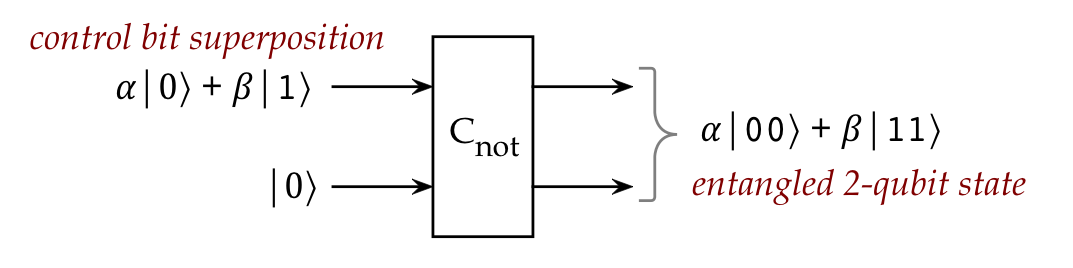
\includegraphics[width=4in]{notes/figs/n07/18cnot1.png}
        \caption{Control bit superposition}
        \label{fig:18cnot1}
    \end{figure}
    
    Then, with $|1\rangle$ reference Figure \ref{fig:19cnot2}.
    
    \begin{figure}
        \centering
        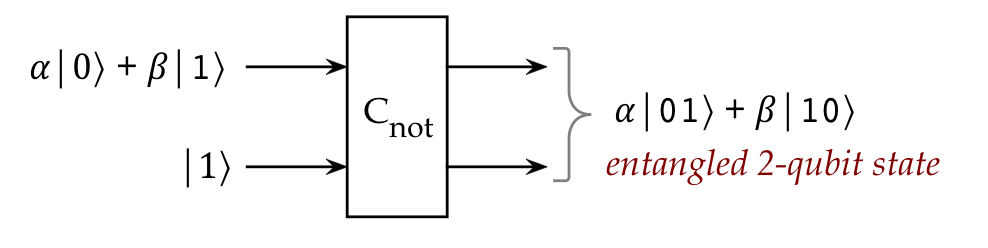
\includegraphics[width=4in]{notes/figs/n07/19cnot2.png}
        \caption{Entangled 2-qubit state}
        \label{fig:19cnot2}
    \end{figure}
    
    Thus, the $C_{\text {Nor }}$ operator can entangle two qubits. In particular, we can now create Bell states, for example with $\alpha=\beta=\frac{1}{\sqrt{2}}$ :
    
    $$
    C_{\text {Nor }}\left(\frac{1}{\sqrt{2}}(|0\rangle+|1\rangle) \otimes|0\rangle\right)=\frac{1}{\sqrt{2}}(|00\rangle+|11\rangle)=\left|\Phi^{+}\right\rangle
    $$
    
    or, more compactly,
    
    $$
    \left|\Phi^{+}\right\rangle=C_{N O}|+, 0\rangle
    $$
    
    Recall that $C_{\text {Nor }}$ is its own inverse, which means
    
    $$
    C_{\text {Nor }}\left|\Phi^{+}\right\rangle=|+, 0\rangle=|+\rangle \otimes|0\rangle
    $$
    
    That is, $C_{\text {Nor }}$ can disentangle some entangled states. $C_{\text {NOr }}$ and Hadamard basis vectors: Let's apply $C_{\text {NOT }}$ to $|+\rangle|+\rangle$ :
    
    $$
    \begin{aligned}
    C_{\text {Nor }}|+\rangle|+\rangle &=(|0\rangle\langle 0|\otimes I+| 1\rangle\langle 1| \otimes X)(|+\rangle \otimes|+\rangle) \\
    &=|0\rangle\langle 0||+\rangle \otimes I|+\rangle+|1\rangle\langle 1||+\rangle \otimes X|+\rangle \\
    &=\frac{1}{\sqrt{2}}|0\rangle \otimes|+\rangle+\frac{1}{\sqrt{2}}|1\rangle \otimes|+\rangle \\
    &=\left(\frac{1}{\sqrt{2}}(|0\rangle+|1\rangle)\right) \otimes|+\rangle \\
    &=|+,+\rangle
    \end{aligned}
    $$
    
    The effect of $C_{N O T}$ on the 2-qubit Hadamard basis vectors:
    
    $$
    \begin{array}{ll}
    C_{\text {NOT }}|+,+\rangle=|+,+\rangle & \text { First unchanged when second is }|+\rangle \\
    C_{\text {Nor }}|-,+\rangle=|-,+\rangle & \text { Same } \\
    C_{\text {Nor }}|+,-\rangle=|-,-\rangle & \text { First fips when second is }|-\rangle \\
    C_{\text {NoT }}|-,-\rangle=|+,-\rangle & \text { Same as above }
    \end{array}
    $$
    
    (See exercise below.) We now see that, without intending so, the second qubit is the "control" qubit with the Hadamard vectors. What to make of this? One has to be careful in assigning intuition to quantum operations. It is not correct to say that (with S-basis) the first bit controls the result of the second. Instead, it's better to think of a operator's result as specific to vectors of interest. And then, one separately analyzes what happens with other vectors. Thus, in designing a quantum circuit, one must be acutely aware of what inputs the circuit will see, and what the output will be. Back to the standard basis, and some notation: There is a convenient notation one uses with the standard basis. Recall the 2-qubit standard basis: $|00\rangle, \quad|01\rangle, \quad|10\rangle, \quad|11\rangle$ One can read the binary digits inside as
    
    $$
    \begin{array}{lll}
    \left|b_{1} b_{0}\right\rangle=|00\rangle & \text { When } b_{1}=0, b_{0}=0 \\
    \left|b_{1} b_{0}\right\rangle=|01\rangle & \text { When } b_{1}=0, b_{0}=1 \\
    \left|b_{1} b_{0}\right\rangle=|10\rangle & \text { When } b_{1}=1, b_{0}=0 \\
    \left|b_{1} b_{0}\right\rangle=|11\rangle & & \text { When } b_{1}=1, b_{1}=0
    \end{array}
    $$
    
    Here, $\circ b_{0}$ is the binary digit in the 0 -th (or $2^{0}$ ) positional location. Likewise, $b_{1}$ is the value in the $2^{1}$ position. The actual numeric value is: $b_{1} 2^{1}+b_{0} 2^{0}$. Thus, one can write the set of standard basis vectors as:
    
    $$
    2 \text {-qubit S-basis }=\left\{\left|b_{1} b_{0}\right\rangle: b_{i} \in\{0,1\}\right\}
    $$
    
    This is probably excessive for the simple 2-qubit basis, but will be useful when we consider the general $n$-qubit basis:
    
    $$
    \mathrm{n} \text {-qubit S-basis }=\left\{\left|b_{n-1} \ldots b_{1} b_{0}\right\rangle: b_{i} \in\{0,1\}\right\}
    $$
    
    The decimal version or numeric value of the binary number is:
    
    $$
    b_{n-1} 2^{n-1}+\ldots+b_{1} 2^{1}+b_{0} 2^{0}=\sum_{i=0}^{n-1} b_{i} 2^{i}
    $$
    
    Note: the indexing begins with 0 , reflecting the appropriate power of $2 .$ Where clarity is needed, commas will be used to separate the binary digits, as in:
    
    $$
    \begin{aligned}
    \left|b_{1}, b_{0}\right\rangle &=\left|b_{1}, b_{0}\right\rangle \\
    |01\rangle &=|0,1\rangle
    \end{aligned}
    $$
    
    In this context, one can write the effect of $C_{N O T}$ on the S-basis vectors as:
    
    $$
    C_{\text {Noт }}\left|b_{1}, b_{0}\right\rangle=\left|b_{1}, b_{1} \oplus b_{0}\right\rangle
    $$
    
    where $\oplus$ is the XOR binary digit operator. Recall (from the Review):
    
    \begin{tabular}{|c|c|c|}
    \hline$b_{1}$ & $b_{0}$ & $b_{1} \oplus b_{0}$ \\
    \hline 0 & 0 & 0 \\
    \hline 0 & 1 & 1 \\
    \hline 1 & 0 & 1 \\
    \hline 1 & 1 & 0 \\
    \hline
    \end{tabular}
    
    XOR is a operator that acts on two binary digits (bits) to produce a bit. One way to describe XOR is that one bit (control) flips the other if the control=1. Note: We have introduced a way to tie Boolean logic to quantum states. This will become important as we start to develop quantum circuits. Lastly, let's show how $C_{\text {Nor }}$ can be derived from its S-basis transformation: Recall that an operator can be described through its effect on a basis: Suppose $A$ is an operator and $\left|v_{1}\right\rangle, \ldots,\left|v_{n}\right\rangle$ is a basis. The operator $A$ is fully specified if one knows $A\left|v_{i}\right\rangle$ for every basis vector $\left|v_{i}\right\rangle$. Then, one can derive the matrix form using the sandwich approach (Module 2):
    
    $$
    A_{i j}=\left\langle v_{i}|A| v_{j}\right\rangle
    $$
    
    Let's see this approach at work with $C_{\text {Nог }}$. That is, our starting point is the desired transformation
    
    $$
    \begin{aligned}
    &C_{\text {Nor }}|00\rangle=|00\rangle \\
    &C_{\text {Nor }}|01\rangle=|01\rangle \\
    &C_{\text {Nor }}|10\rangle=|11\rangle \\
    &C_{\text {Nor }}|11\rangle=|10\rangle
    \end{aligned}
    $$
    
    Now build the matrix:
    
    $$
    C_{\text {NOT }}=\left[\begin{array}{llll}
    \left\langle 00\left|C_{\text {NoT }}\right| 00\right\rangle & \left\langle 00\left|C_{\text {Nor }}\right| 01\right\rangle & \left\langle 00\left|C_{\text {Nor }}\right| 10\right\rangle & \left\langle 00\left|C_{\text {Nor }}\right| 11\right\rangle \\
    \left\langle 01\left|C_{\text {Nor }}\right| 00\right\rangle & \left\langle 01\left|C_{\text {NoT }}\right| 01\right\rangle & \left\langle 01\left|C_{\text {Nor }}\right| 10\right\rangle & \left\langle 01\left|C_{\text {Nor }}\right| 11\right\rangle \\
    \left\langle 10\left|C_{\text {NoT }}\right| 00\right\rangle & \left\langle 10\left|C_{\text {Nor }}\right| 01\right\rangle & \left\langle 10\left|C_{\text {Nor }}\right| 10\right\rangle & \left\langle 10\left|C_{\text {Nor }}\right| 11\right\rangle \\
    \left\langle 11\left|C_{\text {NoT }}\right| 00\right\rangle & \left\langle 11\left|C_{\text {Nor }}\right| 01\right\rangle & \left\langle\mathbf{1 1}\left|\mathbf{C}_{\text {Nor }}\right| 10\right\rangle & \left\langle 11\left|C_{\text {Nor }}\right| 11\right\rangle
    \end{array}\right]
    $$
    
    Which gives us
    
    $$
    C_{\text {NOT }}=\left[\begin{array}{llll}
    1 & 0 & 0 & 0 \\
    0 & 1 & 0 & 0 \\
    0 & 0 & 0 & 1 \\
    0 & 0 & \mathbf{1} & 0
    \end{array}\right]
    $$
    
    For example, the bolded entry is:
    
    $$
    \left\langle 11\left|C_{\text {NoT }}\right| 10\right\rangle=\langle 11 \mid 11\rangle=1
    $$

\subsection{3-qubit examples}

    Let's now look at some examples of applying three tensored 1-qubit operators to three qubits referenced in Figure \ref{fig:20threequbit}.
    
    \begin{figure}
        \centering
        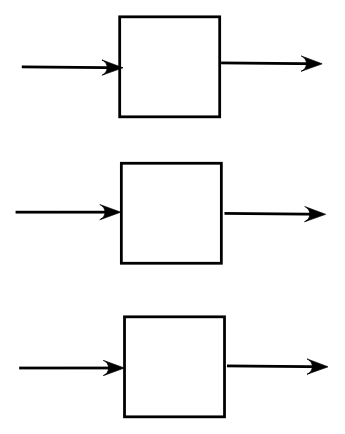
\includegraphics[width=2in]{notes/figs/n07/20threequbit.png}
        \caption{Three tensored 1-qubit operators}
        \label{fig:20threequbit}
    \end{figure}
    
    Example: changing one qubit
    
    $$
    \begin{aligned}
    (I \otimes X \otimes I) \frac{1}{\sqrt{2}}(|000\rangle+|111\rangle) &=\frac{1}{\sqrt{2}}(I \otimes X \otimes I)(|0\rangle \otimes|0\rangle \otimes|0\rangle+|1\rangle \otimes|1\rangle \otimes|1\rangle) \\
    &=\frac{1}{\sqrt{2}}(I|0\rangle \otimes X|0\rangle \otimes I|0\rangle+I|1\rangle \otimes X|1\rangle \otimes I|1\rangle) \\
    &=\frac{1}{\sqrt{2}}(|0\rangle \otimes|1\rangle \otimes|0\rangle+|1\rangle \otimes|0\rangle \otimes|1\rangle) \\
    &=\frac{1}{\sqrt{2}}(|010\rangle+|101\rangle)
    \end{aligned}
    $$
    
    Example: changing one qubit
    
    $$
    \begin{aligned}
    (H \otimes I \otimes I)|000\rangle &=H|0\rangle \otimes|0\rangle \otimes|0\rangle \\
    &=\frac{1}{\sqrt{2}}(|0\rangle+|1\rangle) \otimes|0\rangle \otimes|0\rangle \\
    &=\frac{1}{\sqrt{2}}(|0\rangle|0\rangle|0\rangle+|1\rangle|0\rangle|0\rangle) \\
    &=\frac{1}{\sqrt{2}}(|000\rangle+|100\rangle)
    \end{aligned}
    $$
    
    Example: changing one qubit
    
    $$
    \begin{aligned}
    (I \otimes I \otimes i Y)(|11\rangle \otimes(\alpha|1\rangle-\beta|0\rangle)) &=(I \otimes I \otimes i Y)(|1\rangle \otimes|1\rangle \otimes(\alpha|1\rangle-\beta|0\rangle)) \\
    &=I|1\rangle \otimes I|1\rangle \otimes i Y(\alpha|1\rangle-\beta|0\rangle) \\
    &=|1\rangle \otimes|1\rangle \otimes(\alpha|0\rangle+\beta|1\rangle) \\
    &=\alpha|110\rangle+\beta|111\rangle \\
    Y &=\left[\begin{array}{lc}
    0 & -i \\
    i & 0
    \end{array}\right]
    \end{aligned}
    $$
    
    $$
    \begin{aligned}
    &=I|1\rangle \otimes I|1\rangle \otimes i Y(\alpha|1\rangle-\beta|0\rangle) \\
    &=|1\rangle \otimes|1\rangle \otimes(\alpha|0\rangle+\beta|1\rangle)
    \end{aligned}
    $$
    
    where $Y$ is the Pauli operator and $s 0$
    
    $$
    i Y(\alpha|1\rangle-\beta|0\rangle)=\left[\begin{array}{cc}
    0 & 1 \\
    -1 & 0
    \end{array}\right]\left[\begin{array}{c}
    -\beta \\
    \alpha
    \end{array}\right]=\left[\begin{array}{c}
    \alpha \\
    \beta
    \end{array}\right]=\alpha|0\rangle+\beta|1\rangle
    $$
    
    Example: Changing two qubits
    
    $$
    \begin{aligned}
    (I \otimes X \otimes Z) \frac{1}{\sqrt{2}}(|000\rangle+|111\rangle) &=\frac{1}{\sqrt{2}}(I|0\rangle \otimes X|0\rangle \otimes Z|0\rangle+I|1\rangle \otimes X|1\rangle \otimes Z|1\rangle) \\
    &=\frac{1}{\sqrt{2}}(|0\rangle \otimes|1\rangle \otimes|0\rangle+|1\rangle \otimes|0\rangle \otimes-|1\rangle) \\
    &=\frac{1}{\sqrt{2}}(|010\rangle-|101\rangle)
    \end{aligned}
    $$
    
    Recall the 1-qubit Pauli operator $Z$ :
    
    $$
    Z(\alpha|0\rangle+\beta|1\rangle)=\alpha|0\rangle-\beta|1\rangle
    $$
    
    One can also apply a 2-qubit operator on two of three qubits, with a 1 -qubit operator on the remaining as shown in Figure \ref{fig:21threequbit2}.
    
    \begin{figure}
        \centering
        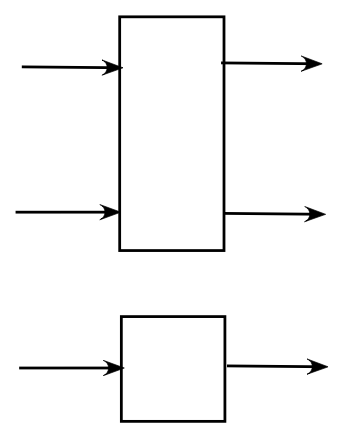
\includegraphics[width=2in]{notes/figs/n07/21threequbit2.png}
        \caption{Apply 2 qubit operator}
        \label{fig:21threequbit2}
    \end{figure}
    
    For example:
    
    $$
    \begin{aligned}
    \left(C_{\text {Nor }} \otimes I\right)\left(\frac{1}{\sqrt{2}}|000\rangle+\frac{1}{\sqrt{2}}|111\rangle\right) &=\frac{1}{\sqrt{2}}\left(C_{\text {NoT }} \otimes I\right)(|00\rangle|0\rangle+|11\rangle|1\rangle) \\
    &=\frac{1}{\sqrt{2}}\left(C_{\text {NOT }}|00\rangle \otimes I|0\rangle+C_{\text {Nor }}|11\rangle \otimes I|1\rangle\right) \\
    &=\frac{1}{\sqrt{2}}(|00\rangle \otimes|0\rangle+|10\rangle \otimes|1\rangle) \\
    &=\frac{1}{\sqrt{2}}(|000\rangle+|101\rangle)
    \end{aligned}
    $$
    
    Another example that will shortly be useful:
    
    $$
    \begin{aligned}
    \left(C_{\text {Nor }} \otimes I\right) \frac{1}{\sqrt{2}}(\alpha|000\rangle+\alpha|011\rangle+\beta|101\rangle+\beta|111\rangle) &=\frac{1}{\sqrt{2}}\left(\alpha C_{\text {Nor }}|00\rangle|0\rangle+\alpha C_{\text {Nor }}|01\rangle|1\rangle+\beta C_{\text {Nor }}|10\rangle|1\rangle+\beta C_{\text {Nor }}|11\rangle|1\rangle\right) \\
    &=\frac{1}{\sqrt{2}}(\alpha|00\rangle|0\rangle+\alpha|01\rangle|1\rangle+\beta|11\rangle|1\rangle+\beta|10\rangle|1\rangle) \\
    &=\frac{1}{\sqrt{2}}(\alpha|000\rangle+\alpha|011\rangle+\beta|111\rangle+\beta|101\rangle)
    \end{aligned}
    $$

\subsection{The no-cloning theorem}

    Consider the possibility of a unitary operator that copies or clones: Suppose $U$ is such an operator as shown in Figure \ref{fig:22clone}.
    
    \begin{figure}
        \centering
        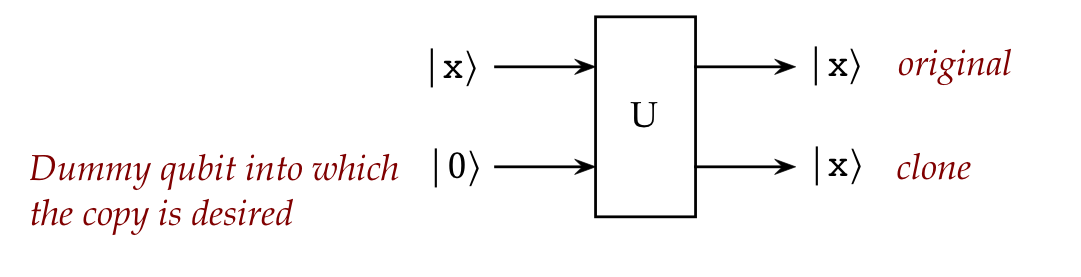
\includegraphics[width=2in]{notes/figs/n07/22clone.png}
        \caption{clone}
        \label{fig:22clone}
    \end{figure}
    
    The target is the top qubit $|x\rangle$ We need a qubit (second one) into which the copy is made. The destination qubit has to be in some state.
    For now, let's assume that state is $|0\rangle$. Since $U$ should work for any qubit state, it must be true that: 
    
    $$
    \begin{aligned}
    &U(|x\rangle \otimes|0\rangle)=|x\rangle \otimes|x\rangle \\
    &U(|y\rangle \otimes|0\rangle)=|y\rangle \otimes|y\rangle
    \end{aligned}
    $$
    
    To get used to an alternative, more compact notation for tensored vectors, let's write this as:
    
    $$
    \begin{aligned}
    &U(|x\rangle|0\rangle)=|x\rangle|x\rangle \\
    &U(|y\rangle|0\rangle)=|y\rangle|y\rangle
    \end{aligned}
    $$
    
    Let
    
    $$
    |\psi\rangle=\frac{1}{\sqrt{2}}(|x\rangle+|y\rangle)
    $$
    
    Then, $U$ should clone this too:
    
    $$
    U(|\psi\rangle|0\rangle)=|\psi\rangle|\psi\rangle
    $$
    
    The right side when simplified becomes
    
    $$
    \begin{aligned}
    |\psi\rangle|\psi\rangle &=\frac{1}{\sqrt{2}}(|x\rangle+|y\rangle) \otimes \frac{1}{\sqrt{2}}(|x\rangle+|y\rangle) \\
    &=\frac{1}{2}(|x\rangle|x\rangle+|x\rangle|y\rangle+|y\rangle|x\rangle+|y\rangle|y\rangle)
    \end{aligned}
    $$
    
    Meanwhile, with the left side
    
    $$
    \begin{aligned}
    U(|\psi\rangle|0\rangle) &=U\left(\frac{1}{\sqrt{2}}(|x\rangle+|y\rangle)|0\rangle\right) \\
    &=U\left(\frac{1}{\sqrt{2}}(|x\rangle|0\rangle)+(|y\rangle|0\rangle)\right) \\
    &=\frac{1}{\sqrt{2}} U(|x\rangle|0\rangle)+\frac{1}{\sqrt{2}} U(|y\rangle|0\rangle) \\
    &=\frac{1}{\sqrt{2}}(|x\rangle|x\rangle)+\frac{1}{\sqrt{2}}(|y\rangle|y\rangle)
    \end{aligned}
    $$
    
    Thus, the two sides are not equal:
    
    $$
    \frac{1}{2}(|x\rangle|x\rangle+|x\rangle|y\rangle+|y\rangle|x\rangle+|y\rangle|y\rangle) \neq \frac{1}{\sqrt{2}}(|x\rangle|x\rangle+|y\rangle|y\rangle)
    $$
    
    This shows that no unitary cloning operator exists that will work on all qubit states. One minor issue: did the above proof rely on the second qubit's initial state being $|0\rangle$? No, $|0\rangle$ just makes it easier to read. The exact same proof would work with any initial state:
    
    $$
    \begin{aligned}
    &U(|x\rangle|v\rangle)=|x\rangle|x\rangle \\
    &U(|y\rangle|v\rangle)=|y\rangle|y\rangle
    \end{aligned}
    $$
    
    Note: there are particular states and operators for which cloning does work, for example:
    
    $$
    \begin{aligned}
    &C_{\text {NOT }}|00\rangle=|00\rangle \\
    &C_{\text {NOT }}|10\rangle=|11\rangle
    \end{aligned}
    $$
    
    Here, the first qubit state gets copied into the second. What's important to keep in mind: The goal of cloning is to reliably copy an unknown quantum state without measuring it. Any measurement of course can destroy the state. Let's revisit the BB-84 protocol: Recall: Alice and Bob use either the $S$ or H bases shown in Figure \ref{23bb84-1}.
    
    \begin{figure}
        \centering
        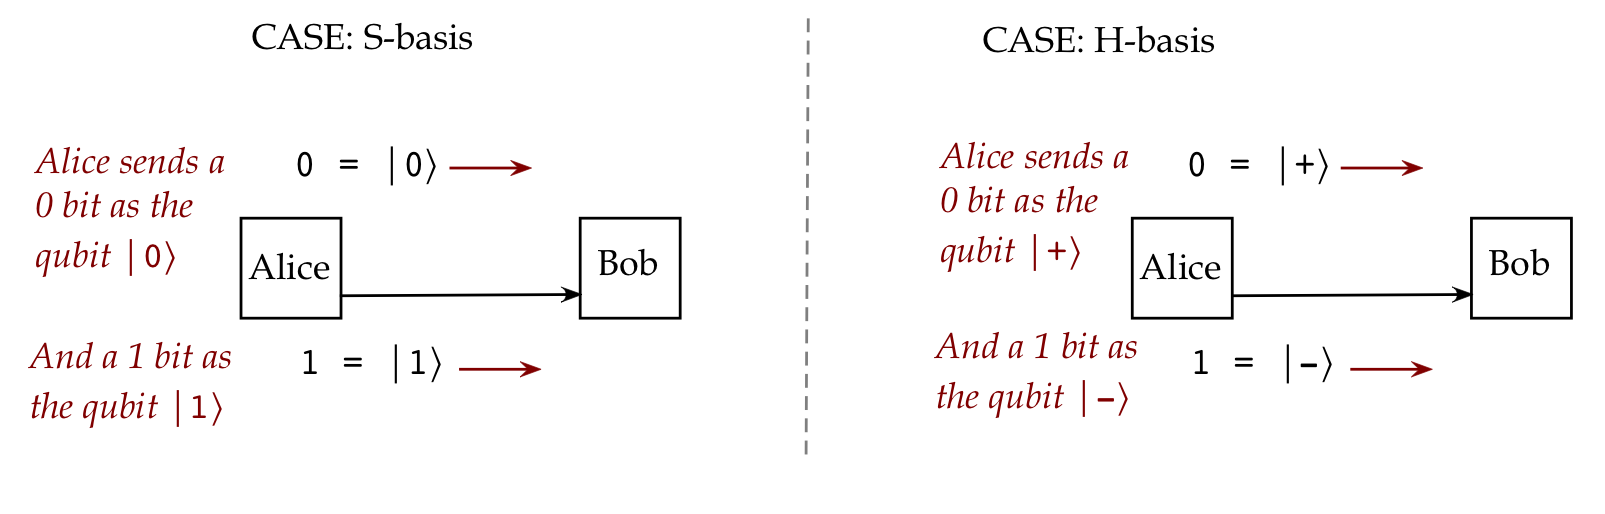
\includegraphics[width=5in]{notes/figs/n07/23bb84-1.png}
        \caption{S and H basis}
        \label{fig:23bb84-1}
    \end{figure}
    
    The security relied on Eve's inability to clone as shown in Figure \ref{fig:24bb84}.
    
    \begin{figure}
        \centering
        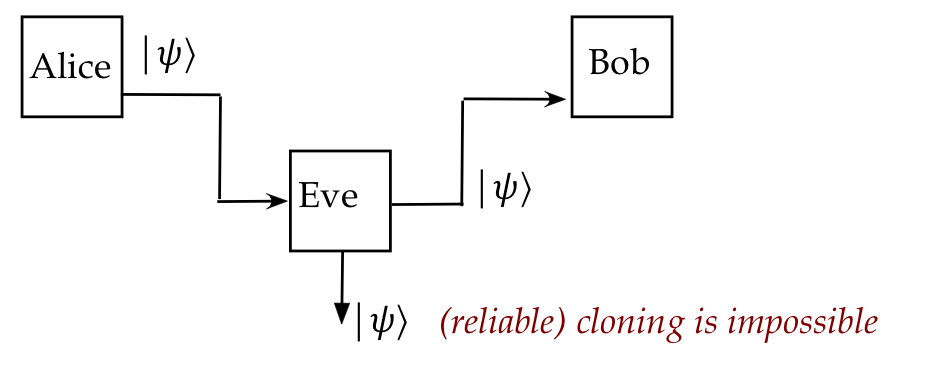
\includegraphics[width=4in]{notes/figs/n07/24bb84.png}
        \caption{Eve cloning impossible}
        \label{fig:24bb84}
    \end{figure}
    
    However, Eve knows the protocol: she only needs an operator to clone four states: $|0\rangle,|1\rangle,|+\rangle,|-\rangle$. For example reference Figure \ref{fig:25bb84-2}.
    
    \begin{figure}
        \centering
        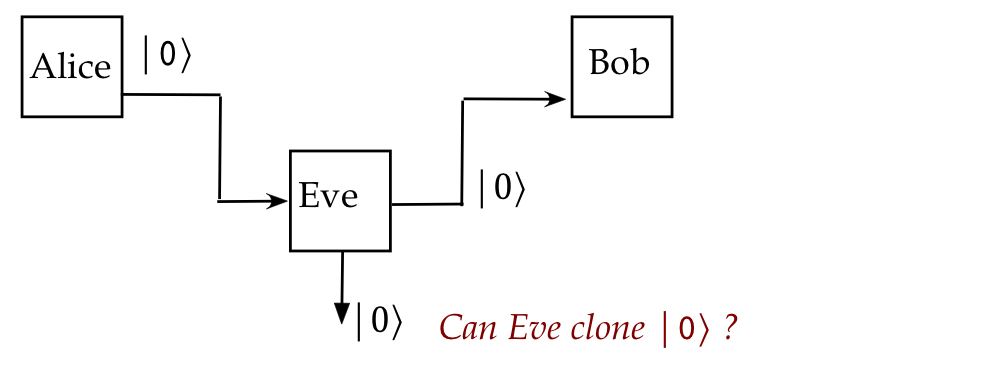
\includegraphics[width=4in]{notes/figs/n07/25bb84-2.png}
        \caption{Eve cloning impossible}
        \label{fig:25bb84-2}
    \end{figure}
    
    Now, there's good and bad news. Let's start with the good. Consider again a supposed unitary operator that clones:
   
    $$
    \begin{aligned}
    &U(|x\rangle|0\rangle)=|x\rangle|x\rangle \\
    &U(|y\rangle|0\rangle)=|y\rangle|y\rangle
    \end{aligned}
    $$
    
    The inner product of the two right sides is:
    
    $$
    \begin{aligned}
    (|x\rangle|x\rangle)^{\dagger}(|y\rangle|y\rangle) &=\langle\langle x|\langle x|| \mid y\rangle| y\rangle\rangle \\
    &=\langle x \mid y\rangle\langle x \mid y\rangle \\
    &=\langle x \mid y\rangle^{2}
    \end{aligned}
    $$
    
    The inner-product of the two left sides:
    
    $$
    \begin{aligned}
    (U(|x\rangle|0\rangle))^{\dagger}(U(|y\rangle|0\rangle)) &=\left(\left\langlex|\langle 0|) U^{\dagger} U(|y\rangle|0\rangle)\right.\right.\\
    &=(\langle x|\langle 0|)(|y\rangle|0\rangle)\\
    &=\langle x \mid y\rangle\langle 0 \mid 0\rangle \\
    &=\langle x \mid y\rangle
    \end{aligned}
    $$
    
    Both inner products must be equal and so
    
    $$
    \langle x \mid y\rangle=\langle x \mid y\rangle^{2}
    $$
    
    This is true only if $\langle x \mid y\rangle=0$ or $\langle x \mid y\rangle=1$. Thus, if the two vectors are not orthogonal, exact cloning is not possible. This is certainly the case with BB-84's use of $|0\rangle$ and $|+\rangle$. However, the Buzek-Hillery algorithm shows that it is possible to clone randomly with a reasonably high chance of success: They use a 3rd qubit as a "helper" qubit and design a 3-qubit unitary $U$ such that:
    
    $$
    \begin{aligned}
    U|0\rangle|0\rangle|0\rangle &=\sqrt{\frac{2}{3}}|0\rangle|0\rangle|0\rangle+\sqrt{\frac{1}{6}}|0\rangle|1\rangle|1\rangle+\sqrt{\frac{1}{6}}|1\rangle|0\rangle|1\rangle \\
    U|1\rangle|0\rangle|0\rangle &=\sqrt{\frac{2}{3}}|1\rangle|1\rangle|1\rangle+\sqrt{\frac{1}{6}}|1\rangle|0\rangle|0\rangle+\sqrt{\frac{1}{6}}|0\rangle|1\rangle|0\rangle
    \end{aligned}
    $$
    
    This achieves cloning of the first qubit with probability $\frac{2}{3}$ if the state is $|0\rangle$ or $|1\rangle$. Then, they show that any state in the first qubit can be cloned in the same way with $U$ :
    
    $$
    U|\psi\rangle|0\rangle|0\rangle=\sqrt{\frac{2}{3}}|\psi\rangle|\psi\rangle|\psi\rangle+\sqrt{\frac{1}{6}}|\psi\rangle\left|\psi^{\perp}\right\rangle\left|\psi^{\perp}\right\rangle+\sqrt{\frac{1}{6}}\left|\psi^{\perp}\right\rangle|\psi\rangle\left|\psi^{\perp}\right\rangle
    $$
    
    The implication for BB-84? Alice and Bob may need more bits to see whether Eve is tampering. Or BB-84 may need to be enhanced in other ways.
    A special and useful case of cloning: While a cloning operator does not exist that will work for general vectors, one can reliably clone special vectors. For example, $C_{N O T} \mathrm{~s}$ can be used to clone standard-basis vectors. We already know this for a single standard-basis qubit state referenced in Figure \ref{fig:26clone2}.
    
    \begin{figure}
        \centering
        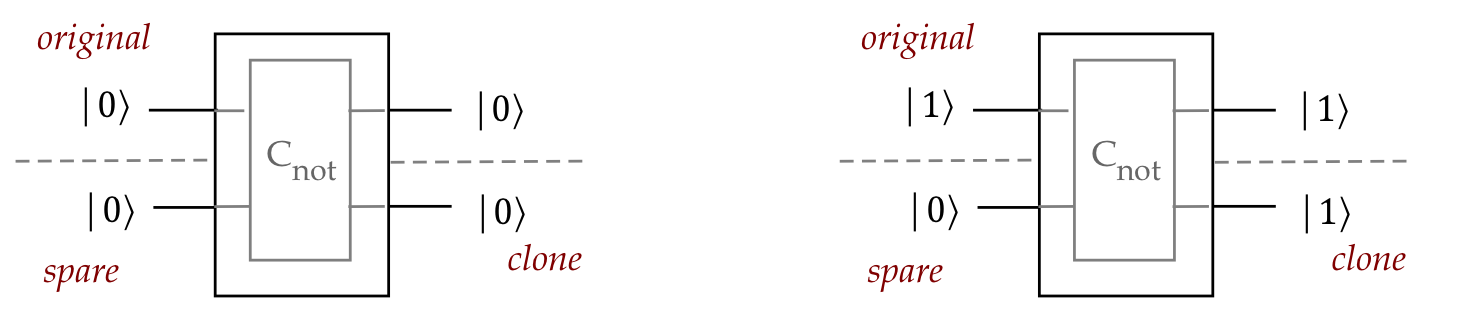
\includegraphics[width=5in]{notes/figs/n07/26clone2.png}
        \caption{single standard basis qubit state clone}
        \label{fig:26clone2}
    \end{figure}
    
    This can be extended to cloning any n-qubit standard basis vector, for example reference Figure \ref{fig:27clone3}.
    
    \begin{figure}
        \centering
        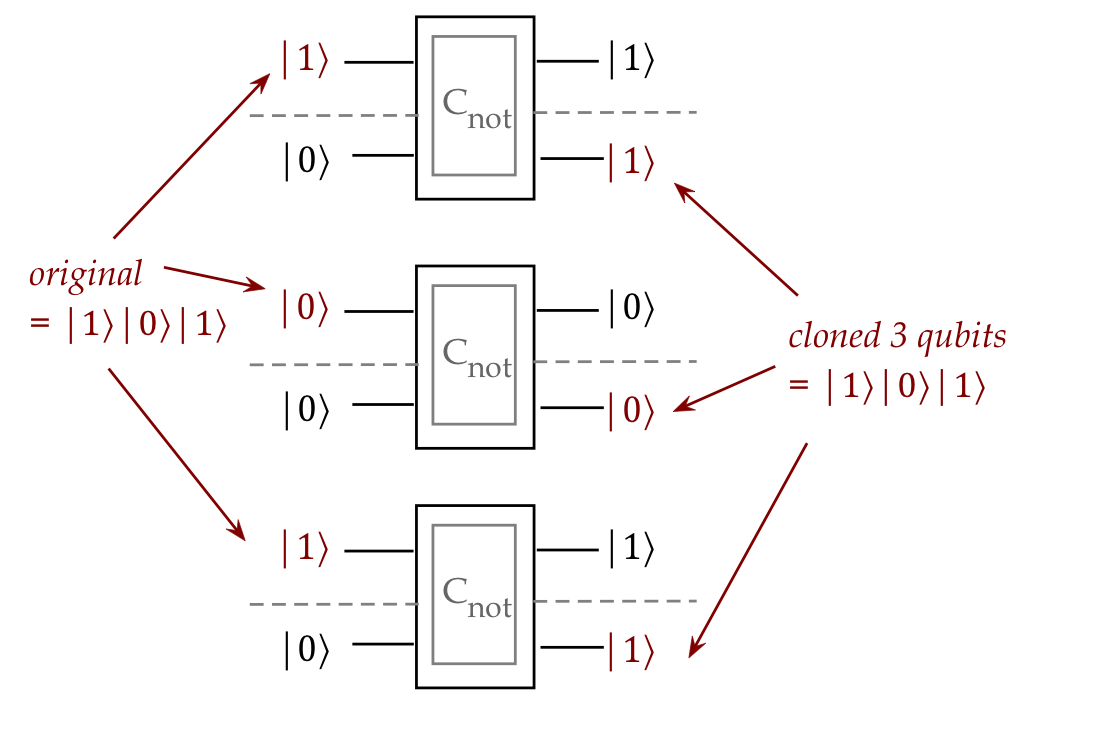
\includegraphics[width=5in]{notes/figs/n07/27clone3.png}
        \caption{n-qubit standard basis vector clone}
        \label{fig:27clone3}
    \end{figure}

\subsection{Quantum teleportation}

    While perfect cloning is not possible, a transfer of an unknown quantum state is possible, even across large distances. This transfer is known as quantum teleportation. It does not achieve cloning because the original state is destroyed. And it needs the "help" of additional classical bits. We'll now outline the steps: Step 1: Alice has a qubit in some unknown state $|\psi\rangle$ shown in Figure \ref{fig:28teleport1}.
    
    \begin{figure}
        \centering
        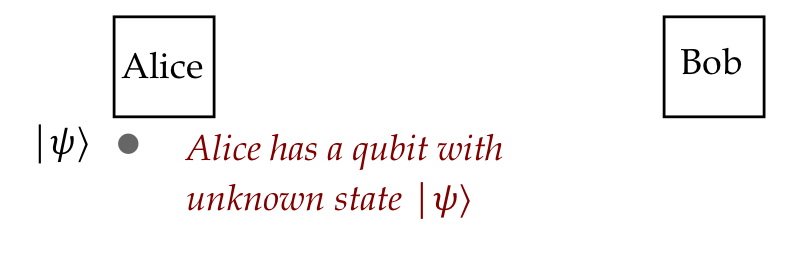
\includegraphics[width=5in]{notes/figs/n07/28teleport1.png}
        \caption{qubit with unknown state}
        \label{fig:28teleport1}
    \end{figure}
    
    The goal is for Alice to have this state transferred to Bob. Let's write the unknown state as:
    
    $$
    |\psi\rangle=\alpha|0\rangle+\beta|1\rangle
    $$
    
    Step 2: Alice and Bob get one qubit each from an entangled Bell state shown in Figure \ref{fig:29teleport2}.
    
    \begin{figure}
        \centering
        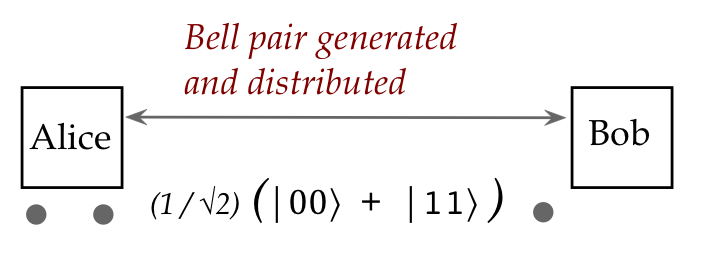
\includegraphics[width=5in]{notes/figs/n07/29teleport2.png}
        \caption{Bell pair generated and distributed}
        \label{fig:29teleport2}
    \end{figure}
    
    Here, we're using the first Bell state:
    
    $$
    \left|\Phi^{+}\right\rangle=\frac{1}{\sqrt{2}}(|00\rangle+|11\rangle)
    $$
    
    Thus, the three qubits are in state
    
    $$
    \begin{aligned}
    |T\rangle &=|\psi\rangle \otimes\left|\Phi^{+}\right\rangle \\
    &=(\alpha|0\rangle+\beta|1\rangle) \otimes \frac{1}{\sqrt{2}}(|00\rangle+|11\rangle) \\
    &=\frac{1}{\sqrt{2}}(\alpha|000\rangle+\alpha|011\rangle+\beta|100\rangle+\beta|111\rangle)
    \end{aligned}
    $$
    
    Step 3: Alice applies $C_{NOT}$ to the two qubits on her side shown in Figure \ref{fig:30teleport3}
    
    \begin{figure}
        \centering
        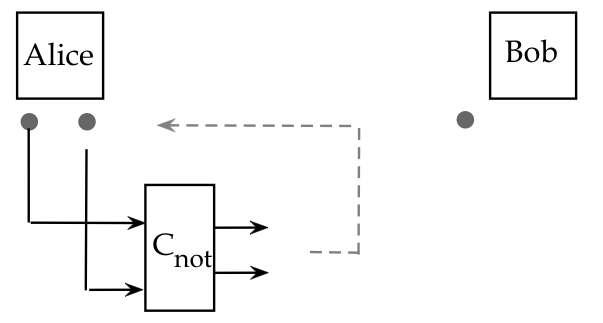
\includegraphics[width=5in]{notes/figs/n07/30teleport3.png}
        \caption{Alice C Not two qubits}
        \label{fig:30teleport3}
    \end{figure}
    
    Since this is a 3-qubit system, Alice is really applying
    
    $$
    \begin{aligned}
    \left(C_{\text {NoT }} \otimes I\right)|T\rangle &=\left(C_{\text {NoT }} \otimes I\right) \frac{1}{\sqrt{2}}(\alpha|000\rangle+\alpha|011\rangle+\beta|100\rangle+\beta|111\rangle) \\
    &=\frac{1}{\sqrt{2}}\left(\alpha C_{\text {NoT }}|00\rangle|0\rangle+\alpha C_{\text {NoT }}|01\rangle|1\rangle+\beta C_{\text {NoT }}|10\rangle|0\rangle+\beta C_{\text {NoT }}|11\rangle|1\rangle\right) \\
    &=\frac{1}{\sqrt{2}}(\alpha|000\rangle+\alpha|011\rangle+\beta|110\rangle+\beta|101\rangle) \\
    & \triangleq\left|T^{\prime}\right\rangle
    \end{aligned}
    $$
    
    Here, we've nameded the result $\left|T^{\prime}\right\rangle$. Step 4: Alice now applies $H \otimes I \otimes I$ shown in Figure \ref{fig:31teleport4}.
    
    \begin{figure}
        \centering
        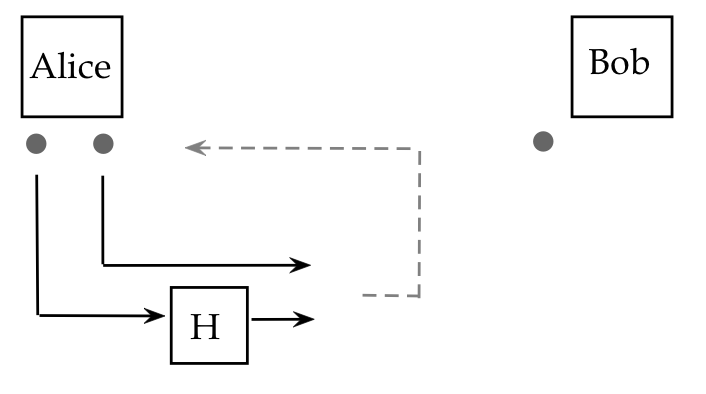
\includegraphics[width=5in]{notes/figs/n07/31teleport4.png}
        \caption{$H \otimes I \otimes I$}
        \label{fig:31teleport4}
    \end{figure}
    
    Thus, the net effect is:
    
    $$
    \begin{aligned}
    \left|T^{\prime \prime}\right\rangle=&(H \otimes I \otimes I)\left|T^{\prime}\right\rangle \\
    =&(H \otimes I \otimes I) \frac{1}{\sqrt{2}}(\alpha|000\rangle+\alpha|011\rangle+\beta|110\rangle+\beta|101\rangle) \\
    =&(H \otimes I \otimes I) \frac{1}{\sqrt{2}}(\alpha|000\rangle+\alpha|011\rangle+\beta|110\rangle+\beta|101\rangle) \\
    =& \frac{1}{2}(\alpha|000\rangle+\alpha|100\rangle+\alpha|011\rangle+\alpha|111\rangle\\
    &\beta|010\rangle-\beta|110\rangle+\beta|001\rangle-\beta|101\rangle) \\
    =& \frac{1}{2}(\alpha|000\rangle+\beta|001\rangle+\alpha|011\rangle+\beta|010\rangle\\
    &\alpha|100\rangle-\beta|101\rangle+\alpha|111\rangle-\beta|110\rangle)
    \end{aligned}
    $$
    
    Which simplifies to:
    
    $$
    \begin{aligned}
    \left|T^{\prime \prime}\right\rangle=& \frac{1}{2}|00\rangle(\alpha|0\rangle+\beta|1\rangle) \\
    +& \frac{1}{2}|01\rangle(\alpha|1\rangle+\beta|0\rangle) \\
    +& \frac{1}{2}|10\rangle(\alpha|0\rangle-\beta|1\rangle) \\
    &+\frac{1}{2}|11\rangle(\alpha|1\rangle-\beta|0\rangle)
    \end{aligned}
    $$
    
    Step 5: Alice measures both her qubits in the standard basis shown in Figure \ref{fig:32teleport5}.
    
    \begin{figure}
        \centering
        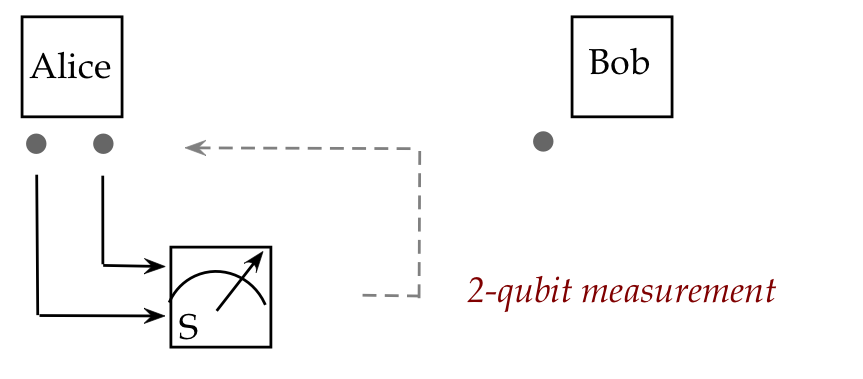
\includegraphics[width=5in]{notes/figs/n07/32teleport5.png}
        \caption{Alice measures}
        \label{fig:32teleport5}
    \end{figure}
    
    Alice's 2-qubit measurement occurs with the projectors
    
    $$
    \begin{aligned}
    &P_{00}=|00\rangle\langle 00| \\
    &P_{01}=|01\rangle\langle 01| \\
    &P_{10}=|10\rangle\langle 10| \\
    &P_{11}=|11\rangle\langle 11|
    \end{aligned}
    $$
    
    In the 3 -qubit system with $\left|T^{\prime \prime}\right\rangle$ as the state, the projectors are then
    
    $$
    \begin{aligned}
    &P_{00} \otimes I=|00\rangle\langle 00| \otimes I \\
    &P_{01} \otimes I=|01\rangle\langle 01| \otimes I \\
    &P_{10} \otimes I=|10\rangle\langle 10| \otimes I \\
    &P_{11} \otimes I=|11\rangle\langle 11| \otimes I
    \end{aligned}
    $$
    
    Alice then observes one of four S-basis states: $|00\rangle,|01\rangle,|10\rangle$ or $|11\rangle$. However, the four possible 3-qubit outcomes of Alice's measurement are:
    
    $$
    \begin{aligned}
    &|00\rangle \otimes(\alpha|0\rangle+\beta|1\rangle) \\
    &|01\rangle \otimes(\alpha|1\rangle+\beta|0\rangle) \\
    &|10\rangle \otimes(\alpha|0\rangle-\beta|1\rangle) \\
    &|11\rangle \otimes(\alpha|1\rangle-\beta|0\rangle)
    \end{aligned}
    $$
    
    That is, Bob will end up with one of the four qubit states on the right. Step 6: Alice communicates a classical value to tell Bob which basis state resulted from measurement shown in Figure \ref{fig:33teleport6}.
    
    \begin{figure}
        \centering
        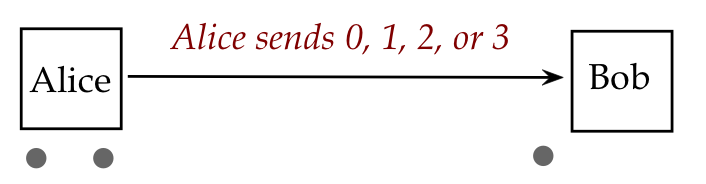
\includegraphics[width=5in]{notes/figs/n07/33teleport6.png}
        \caption{Alice communicates}
        \label{fig:33teleport6}
    \end{figure}
    
    If the outcome is $|00\rangle$, she sends "0". If $|01\rangle$, she sends "1". If $|10\rangle$, she sends "2". If $|11\rangle$, she sends "3". This single message counts as two classical binary digits (bits). When Bob receives this information, he'll know which of four unknown states his qubit is in, but this is not the goal. $\triangleright$ Recall: neither of them know $\alpha, \beta$. Bob will now transform his qubit without measuring with the goal of transforming it to $\alpha|0\rangle+\beta|1\rangle$. The following 1-qubit transforms achieve the goal:
    
    $$
    \begin{array}{rlr}
    I(\alpha|0\rangle+\beta|1\rangle) & =(\alpha|0\rangle+\beta|1\rangle) & \text { if Alice sent "0" } \\
    X(\alpha|1\rangle+\beta|0\rangle) & =(\alpha|0\rangle+\beta|1\rangle) & \text { if Alice sent "1" } \\
    Z(\alpha|0\rangle-\beta|1\rangle) & =(\alpha|0\rangle+\beta|1\rangle) & \text { if Alice sent "2" } \\
    i Y(\alpha|0\rangle+\beta|1\rangle) & =(\alpha|0\rangle+\beta|1\rangle) & \text { if Alice sent "3" }
    \end{array}
    $$
    
    Step 7: Bob applies one of four transforms depending on which classical message he receives as shown in Figure \ref{fig:34teleport7}.
    
    \begin{figure}
        \centering
        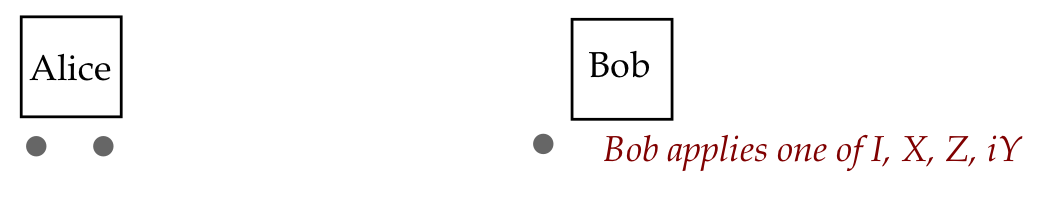
\includegraphics[width=5in]{notes/figs/n07/34teleport7.png}
        \caption{Alice communicates}
        \label{fig:34teleport7}
    \end{figure}
    
    Note: Since this is a 3-qubit system, Bob is really applying one of
    
    $$
    \begin{array}{cc}
    (I \otimes I) \otimes I & \text { for "0" } \\
    (I \otimes I) \otimes X & \text { for "1" } \\
    (I \otimes I) \otimes Z & \text { for "2" } \\
    (I \otimes I) \otimes i Y & \text { for "3" }
    \end{array}
    $$
    
    At this point: Bob's qubit is in the state $\alpha|0\rangle+\beta|1\rangle$, the original state of Alice's qubit. Alice's qubit state is destroyed (measured). Notice the key steps: Alice performs transforms where the numbers $\alpha, \beta$ apply to the entire three-qubit state. When she measures, the outcome is a standard vector, leaving $\alpha, \beta$ applying to Bob's qubit. Bob applies a non-destroying (unitary) transform to adjust the qubit to Alice's original state. He needs to know which transform to apply: this comes from the classical message. Thus, one could say that the state got transported with the help of a classical message. What does it all mean? Is this a fair use of the "beam me up" term teleportation? Some skepticism: It's not clear that the approach could work for anything that constitutes matter. Even if matter could be unitarily transformed, how would the entangled precursor be created? Even if a single molecule could be recreated, how can one recreate the ensemble state of a collection of atoms? On the other hand. It is true that only information was transferred. A full, unknown quantum state does in fact get recreated. Recent experiments (example) show that atoms can be created as entangled pairs. What do you think?

\subsection{Hermitian theory}

    Let's recall what we know about Hermitians and measurement so far: A Hermitian matrix "packages" projectors along with eigenvalues. For example, suppose a multi-qubit measurement consists of projectors $P_{1}, P_{2}, \ldots, P_{k}$. Then, for any choice of real numbers $\lambda_{1}, \ldots, \lambda_{k}$, the operator
    
    $$
    A=\sum_{i} \lambda_{i} P_{i}
    $$
    
    is Hermitian. In the simplest case, every projector is just an outer-product
    
    $$
    P_{i}=\left|\phi_{i}\right\rangle\left\langle\phi_{i}\right|
    $$
    
    where $\phi_{i}$ is a basis-vector of the measuring device. In this case, we could write
    
    $$
    A=\sum_{i} \lambda_{i} P_{i}=\lambda_{i}\left|\phi_{i}\right\rangle\left\langle\phi_{i}\right|
    $$
    
    Here, the $\phi_{i}$ 's now become the eigenvectors of $A$, with associated eigenvalues $\lambda_{i}$ by this construction. Then, the single operator $A$ contains all the information for the measurement: the projectors and the eigenvalues that correspond to real physical observed values. Constructing multi-qubit Hermitians from smaller Hermitians: Recall: one can construct some larger projectors one qubit at a time:
    
    $$
    \begin{aligned}
    |01\rangle\langle 01| &=P_{01} & & \text { Projector for }|01\rangle \text { outcome } \\
    &=P_{0} \otimes P_{1} & & \text { Tensor product of smaller projectors } \\
    &=\left(I \otimes P_{1}\right)\left(P_{0} \otimes I\right) & & \text { Apply } P_{0} \text { first, then } P_{1} \\
    &=(I \otimes|1\rangle\langle 1|)(|0\rangle\langle 0| \otimes I) & & \text { The smaller ones as outerproducts }
    \end{aligned}
    $$
    
    In the same way, because Hermitians tensor into larger Hermitians, one can construct a larger Hermitian out of smaller ones:
    
    $$
    \begin{aligned}
    A &=B \otimes C & & 2 \text {-qubit Hermitian } A \text { from tensoring 1-qubit Hermitians } \\
    &=(I \otimes C)(B \otimes I) & & \text { Decomposition into stages }
    \end{aligned}
    $$
    
    How does any of this matter? For quantum computing algorithms, Hermitians do not really matter because projectors are sufficient. Thus, the eigenvalues in the "packaging" do not matter as long as different projectors have different eigenvalues. However, quantum computing hardware uses physical devices governed by quantum mechanics. In this case, the actual physical observed values are the eigenvalues. These come from the underlying physics of the system. When tensoring smaller systems, the resulting larger system's eigenvalues can be expressed as products of the smaller system's eigenvalues. Hermitians corresponding to different measurement types can also be deployed in sequence: In this case, they may or may not share eigenvectors. If the eigenvectors are the same, the measurements commute. In this case, the second measurement's outcome will be the same as the first's outcome: There is certainty in the second outcome. Otherwise, the first measurement will result in probabilistic outcomes for the second: Heisenberg's uncertainty principle. Hermitian theory is useful in analysis: For example, one can use the Hermitian sandwich to calculate averages, what one should see in repeated measurements of a physical system.

\end{document}